
\documentclass{report}
\usepackage{amsmath,amsfonts,amssymb,graphicx,tikz,fancyhdr,fancybox,boxedminipage,palatino}
\usepackage[utf8]{inputenc}
\usepackage{anysize}
\usepackage[cyr]{aeguill}
\usepackage{fancyhdr}
\usepackage{mathrsfs}
\usepackage{enumerate} 

%usepackage{amssymb}
\usepackage{amsmath}
\usepackage{amsthm}
\usepackage[utf8]{inputenc}
\usepackage[T1]{fontenc}
\usepackage{lmodern}
\usepackage{ae}
\usepackage{enumerate}
\usepackage[frenchb]{babel}
\usepackage{graphicx}
\usepackage[top=4cm, bottom=4cm, left=3cm, right=3cm]{geometry}

\usepackage{tikz,tkz-tab} % pour les tableaux de variations et bien plus

\usepackage{tikz}
\usetikzlibrary{shapes}


%\setlength{\baselineskip}{1,5\baselineskip}
\renewcommand{\baselinestretch}{1.19}%\small\normalsize
\newtheorem{Def}{Définition}[subsection]
\newtheorem{Ex}{Exemple}[subsection]
\newtheorem{The}{Théorème}[subsection]
\newtheorem{Prop}{Proposion}[subsection]
\newtheorem{Lem}{Lemme}[subsection]
\newtheorem{Cor}{Corollaire}[subsection]
\newtheorem{Rem}{Remarque}[subsection]

\renewcommand{\thesection}{\arabic{section}}
\renewcommand{\thesubsection}{\arabic{section}.\arabic{subsection}}


%\documentclass[a4paper,12pt]{report}
%\usepackage[T1]{fontenc}
%\usepackage[utf8]{inputenc}
%\usepackage[utf8]{inputenc}
%\usepackage[french]{babel}
%\usepackage{hyperref}
%\usepackage{amsmath}
%\usepackage{amsthm}
%\usepackage{amsfonts}
%\usepackage{amssymb}
%\usepackage{color}
%\usepackage{graphicx}
\topmargin=-.5in \textheight=9.in\leftmargin=-.2in
\renewcommand{\baselinestretch}{1.4} 
\usepackage{fancyhdr}
\usepackage{lastpage}
\usepackage{geometry}
\geometry{left=3.5cm,right=3.5cm,top=3cm,bottom=3cm}



\newcommand*\chancery{\fontfamily{pzc}\selectfont}
\usepackage{courier}

	% --- Indication des couleurs (pour couleur #1, pour nb #2)
\newcommand{\couleurnb}[2]{#1}
%-------------------------------------------------------------
%Les chapitre
% Police par defaut
%%%%%%%%%%%%%%%%%%%%%%%%%%%%%%%%%%%%%%%%%%%%%%%%%%%%%%%%%
%%%%%%%%%%%%%%%%%%%%%%  For Section
% Align? ? gauche, suivi d'un filet horizontal, l?g?rement dans la marge
\newcommand{\ls}{\vskip -1.5ex\nobreak
	\noindent\hrule height 2pt
	\vskip 0.5ex\nobreak
	\noindent\hrule height 1pt
	\vskip 3ex}
%%%%%%%%%%%%%%%%%%%%%%  For Chapter
\makeatletter
\def\thickhrulefill{\leavevmode \leaders \hrule height 1ex \hfill \kern \z@}
\def\@makechapterhead#1{%
	%\vspace*{50\p@}%
	\vspace*{10\p@}%
	{\parindent \z@ \centering \reset@font
		\thickhrulefill\quad
		\scshape \@chapapp{} \thechapter
		\quad \thickhrulefill
		\par\nobreak
		\vspace*{10\p@}%
		\interlinepenalty\@M
		\hrule
		\vspace*{10\p@}%
		\Huge \bfseries #1\par\nobreak
		\par
		\vspace*{10\p@}%
		\hrule
		%\vskip 40\p@
		\vskip 100\p@
	}}
	\def\@makeschapterhead#1{%
		%\vspace*{50\p@}%
		\vspace*{10\p@}%
		{\parindent \z@ \centering \reset@font
			\thickhrulefill
			\par\nobreak
			\vspace*{10\p@}%
			\interlinepenalty\@M
			\hrule
			\vspace*{10\p@}%
			\Huge \bfseries #1\par\nobreak
			\par
			\vspace*{10\p@}%
			\hrule
			%\vskip 40\p@
			\vskip 40\p@
		}}	
		\lhead{Sur la fonction Gamma d'Euler}
		\rhead{}
		%\cfoot{Faculté des Sciences et Techniques Fès}
		%\lfoot{Ayoub Guemia}
		%\rfoot{\thepage / \pageref{LastPage}}
		

\usepackage{pdfpages}

\begin{document}

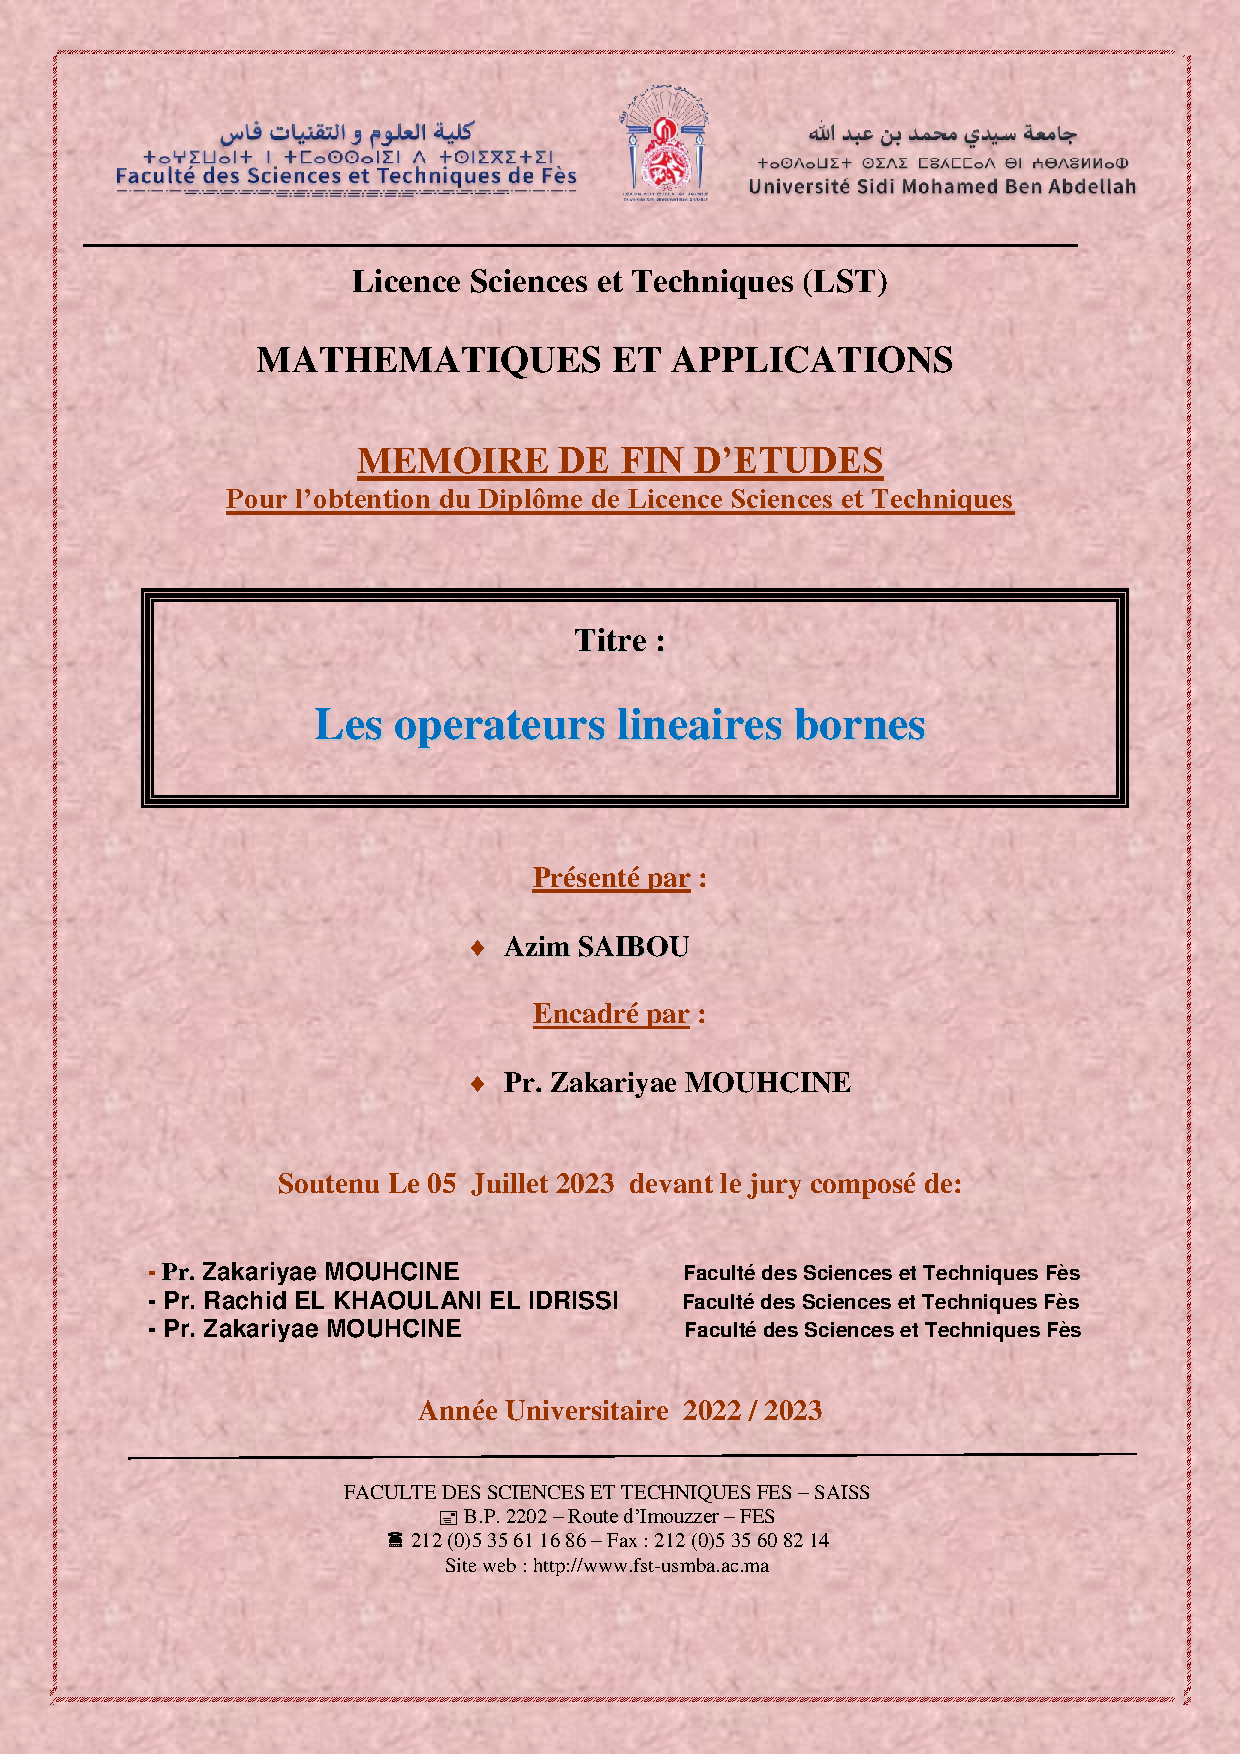
\includepdf[pages=-]{PageDeGarde.pdf}

\sffamily



%%%%%%%%%%%% Debut Remerciements %%%%%%%%%%%%%%
\chapter*{REMERCIEMENT}
 
\textit{J'aimerais en premier lieu remercier mon Dieu Allah qui m'a donné la volonté et le courage pour la réalisation de ce travail.}

\vspace{0.8cm}

\textit{Je tiens à exprimer mon énorme remerciement et mes respects les plus profonds à : 
Mon encadrant pédagogique Mr Zakariyae MOUHCINE, Professeur à l'FST de Fès, pour son encadrement, ses conseils, son aide et son soutien tout au long du projet.}

\vspace{0.8cm}

\textit{Je voudrais également remercier les membres du jury d'avoir accepter d'évaluer ce travail et pour toutes leurs remarques et critiques.}

\vspace{0.8cm}


\textit{Je tiens à remercier vivement toutes les personnes, qui, de près ou de loin, se sont impliquées dans la réalisation de ce projet, tant par leur présence, leurs conseils, leur disponibilité et leur soutien opérationnel, que professionnel.
}

\vspace{0.8cm}

\textit{Enfin, un remerciement spécial à mes parents pour leurs soutiens et leurs sacrifices. Ainsi, que toute personne ayant contribué de près ou de loin à la réussite de ce travail, trouve ici l’expression de mes sentiments les meilleurs.}

\vspace{0.7cm}

\hfill\textit{Azim SAIBOU}



%%%%%%%%%%%%%% Debut Resume %%%%%%%%%%%%%%%%%%%%
\chapter*{RÉSUMÉ}

\vspace{1.5cm}

En mathématiques, un opérateur linéaire (ou plus simplement un opérateur) est une fonction entre deux espaces vectoriels qui est linéaire sur son domaine de définition.\\

Cette notion est particulièrement utile non seulement en analyse vectorielle et fonctionnelle mais aussi en physique quantique.

\vspace{0.8cm}

{\textbf{Keywords:} \textit{Opérateurs; Opérateurs linéaires; Opérateurs adjoints; Produits scalaires.}



% ------------------------------------------------------------------()
\newpage
	

\tableofcontents
\newpage



\chapter*{
\begin{large}{
\textbf{LES OPÉRATEURS  LINÉAIRES BORNES
\textbf{%\includegraphics[height=1cm]{trait}
}}}\end{large}
}





% ------------------------Premiere partie----------------------------------------%
% -------------------------------------------------------------------------------%
% -------------------------------------------------------------------------------%
% -------------------------------------------------------------------------------%


\section{\underline{OPÉRATEURS LINÉAIRES BORNES}}
 Tout au long de cet exposé, on travaillera sur un corps $\mathbb{K}$, qui sera soit $\mathbb{R}$ soit $\mathbb{C}$. Soient $E$ et $F$ deux espaces normes sur $\mathbb{K}$


\subsection{\underline{Définitions et propriétés}}


\begin{Def} On appelle opérateur linéaire de $E$ dans $F$ toute application $A$ de $E$ dans $F$ vérifiant $\forall x, y \in E$ et $\lambda \in \mathbb{K}$ :
	\begin{enumerate}
	\item $A(x + y) = A(x) + A(y)$.
	\item $A(\lambda x) = \lambda A(x)$
	\end{enumerate}
\end{Def}



\begin{Ex}
L'opérateur identité de $E$ dans $E$ est un banal exemple d'opérateur linéaire.
\end{Ex}


\begin{Def}
Soit $T: (E, \lVert . \rVert_{E})  \rightarrow (F, \lVert . \rVert_{F})$ une application.\\ On dit que $T$ est bornée si elle envoie toutes les parties bornées de $E$ sur des parties bornées de $F$ i.e. $T$(tout bornée) est bornée.
\end{Def}


\textbf{\underline{Remarque :}} Soit $T: (E, \lVert . \rVert_{E})  \rightarrow (F, \lVert . \rVert_{F})$ une application. $T$ est bornée  veut dire, pour tout $\epsilon > 0$, il existe $\delta > 0$ tel que 
			\begin{align*}
			  \text{pour tout}\,\, x \in E : \lVert x \rVert_{E} \leq \epsilon \,\,\text{implique}\,\, \lVert T(x) \rVert_{F} \leq \delta 
			\end{align*}


\begin{Prop}
Soit $A$ une application linéaire de $E$ dans $F$, alors $A$ est bornée si et seulement s'il existe une constante $M > 0$ tel que pour tout $x$ dans $E$.
			\begin{align*}
				\lVert A(x) \rVert_{F} \leq M \lVert x \rVert_{E}
			\end{align*}
\end{Prop}
\begin{proof}
$\newline$
\fbox{$(\Rightarrow)$} Si $A$ est une application est bornée, alors il existe $M > 0$, tel que
			\begin{align*}
				\lVert A(x) \rVert_{F} \leq M, \,\,\text{pour tout}\,\, x \in \overline{B_{E}}(0,1)
			\end{align*}
soit $x \in E - \{0\}$, alors $\frac{x}{\lVert x \rVert_{E}} \in \overline{B_{E}}(0,1)$. Cela nous donne 
			\begin{align*}
				\lVert A(x) \rVert_{F} \leq M \lVert x \rVert_{E}, \,\,\text{pour tout}\,\, x \in E.
			\end{align*}

\fbox{$(\Leftarrow)$} Soit $\epsilon > 0$, pour tout $x \in E$, tel que $\lVert x \rVert_{E} \leq \epsilon$, on obtient 
			\begin{align*} 
				\lVert A(x) \rVert_{F} \leq M \epsilon 
			\end{align*}
ça signifie $\delta = M \epsilon$, d'où $A$ est bornée.
\end{proof}


% ----------------------------------------------------

\begin{Def}
(Opérateur borné). On appelle un opérateur  borné de $E$ dans $F$ toute application linéaire bornée de $E$ dans $F$. En d'autres termes, s'il existe une constante $M > 0$ tel que pour tout $x$ dans $E$ 
			\begin{align*}\lVert A(x) \rVert_{F} \leq M \lVert x \rVert_{E}\end{align*}
\end{Def}


\textbf{\underline{\textit{Notation:}}} On note $\mathscr{L}(E, F)$ l'espace vectoriel des applications linéaires continues de E dans F, on note $\mathscr{L}(E) = \mathscr{L}(E, E)$\\



\begin{Ex}
On munit l'espace $E = L^{2}([0,1], \mathbb{R})$ de la norme $\lVert . \rVert_{2}$ Soit $\phi \in E$, on définit l'opérateur $T_{\phi} : E \rightarrow \mathbb{R}$ par : 
			\begin{align*}T_{\phi}(f) = \int_{0}^{1} f(t)\phi(t) dt\end{align*}	
\fbox{Montrons que $T_{\phi} \in L(E, F)$}	\\
En effet, c'est clair que $T_{\phi}$ est linéaire. Par l'inégalité de Cauchy Schwarz, on a :	
			\begin{align*}
				|T_{\phi}| &\leq \int_{0}^{1} |f(t)| |\phi(t)| dt	\\
					      &\leq \sqrt{\int_{0}^{1} |f(t)|^{2} dt}	 \sqrt{|\phi(t)|^{2} dt}
			\end{align*}
Alors l'opérateur $T_{\phi}(f)$ est  borné.
\end{Ex}



\subsection{\underline{ Continuité des opérateurs linéaires}}




\begin{Def}
Soit $a \in E$ et $F: (E, \lVert . \rVert_{E})  \rightarrow (F, \lVert . \rVert_{F})$. On dit que $F$ est continu au point $a \in E$, si et seulement si, pour tout $\epsilon > 0$, il existe $\delta > 0$, pour $x \in E$, on a 
			\begin{align*}
			|| x - a ||_{E} < \delta \,\,\text{implique}\,\, || F(x) - F(a)||_{F} < \epsilon
			\end{align*}
\end{Def}




\begin{The} \label{v:2}
Soit $A$ une application linéaire de $E$ dans $F$ alors $A$ est continue si et seulement si elle est bornée.
\end{The}
\begin{proof}
$\newline$
\fbox{$(\Rightarrow)$} Comme  l'opérateur $A$ est continu au point $0$, alors, il existe $\rho > 0$, tel que
		
		\begin{align*}
		||A(x)||_{F} \le 1, 	\,\,\text{pour tout}\,\, x \in \overline{B}(0,\rho) 
		\end{align*}

Pour tout $\epsilon > 0$ et $x \in E$, tel que $||x|| \le \epsilon$, alors $\frac{\rho}{\epsilon} \in \overline{B}(0,\rho)$, donc
		\begin{align*}||A(\frac{\rho}{\epsilon} x)|| \le 1\end{align*}
ou encore	
		\begin{align*} ||A(x)||_{F} \le \frac{\epsilon}{\rho} \end{align*}
Cela signifie que $\delta = \frac{\epsilon}{\rho}$, ce qui implique l'opérateur $A$ est borné.

\fbox{$(\Leftarrow)$} Supposons que l'opérateur $A$ est  borné. Alors il existe une constante $M > 0$, tel que
			\begin{align*}
			||A(x)||_{F} \leq M ||x||_{E}		, pour tout x \in E
			\end{align*}
Pour $x, y \in E$, on a : 
			\begin{align*}||A(x)-A(y)||_{F} = ||A(x-y)|| \le M ||x-y||_{E}\end{align*}
Cela signifie que l'opérateur $A$ est $M$-Lipschitzienne, donc $A$ est continu sur $E$.

\end{proof}


% -------------------------------------------------

\begin{The}
Soit $A \in \mathscr{L}(E,F)$. Alors, les propositions suivantes sont équivalentes :
	\begin{enumerate}
	\item $A$ est continu sur $E$.		
	\item $A$ est continu en $0_{E}$			
	\item $A$ est borné sur $\overline{B_{E}}(0,1)$			
	\item $A$ est borné sur $S(0,1)$		
	\item Il existe $M \in \mathbb{R}^{+}$ tel que $\forall x \in E$, $||Ax||_{F} \le M ||x||_{E}$	
	\item $A$ est uniformément continu sur $E$.
	\end{enumerate}
\end{The}
\begin{proof}
$\newline$
\fbox{$(1) \Rightarrow (2)$}, est évidente.		\\

\fbox{$(2) \Rightarrow (3)$}, si $A$ est continu en $0_{E}$, alors il existe $\delta > 0$, tel que 
			\begin{align*}
				\,\,\text{si}\,\, x \in \overline{B_{E}}(0,\delta)  \,\,\text{:}\,\,  A(x) \in \overline{B_{F}}(0,1)
			\end{align*}
Soit $x \in \overline{B_{E}}(0,\delta)$, alors $\delta > 0$, donc $A(x) \in \overline{B_{F}}(0,\delta)$, comme $A \in \mathscr{L}(E,F)$, alors 		
			\begin{align*}
				\forall x \in \overline{B_{E}}(0,1), A(x) \in \overline{B_{F}}(0,\frac{1}{\delta})	
			\end{align*}
donc $A$ est  borné sur $\overline{B_{E}}(0,1)$.	\\

\fbox{$(3) \Rightarrow (4)$}, est évidente.	\\

\fbox{$(4) \Rightarrow	(5)$}, si A est  borné sur $S(0,1)$, alors il existe $M > 0$, tel que 	\\
			\begin{align*}
				\forall x \in S(0,1), ||A(x||_{F} \le M
			\end{align*}
Soit $x \in E$, avec $x\neq 0$, on a $\frac{x}{||x||_{E}} \in S(0,1)$, donc 		\\

			\begin{align*}
				||A(\frac{x}{||x||_{E}})||_{F} \le M
			\end{align*}
d'où 			
			\begin{align*}
				\forall x \in E, ||A(x)||_{F} \le M ||x||_{E}
			\end{align*}

\fbox{$(5) \Rightarrow	(6)$}, Soit $x, y \in E$, on a 

			\begin{align*}
				||A(x) - A(y)||_{F} = ||A(x-y)||_{F} \le M ||x-y||_{E}
			\end{align*}

Alors $A$ est M-Lipschitzien, d'où $A$ est uniformément continu sur $E$.		\\

\fbox{$(6) \Rightarrow (1)$}, est évident.		
\end{proof}


% ------------------------------------------------(5)

\begin{The}Soit $A$ un opérateur borné de $E$ dans $F$. Posons :	
			\begin{align*} N_{1} &= \sup_{x \in E- \{0\}} \frac{||Ax||_{F}}{||x||_{E}} 	\\
					N_{2} &= \sup_{x \in S(0,1)} ||Ax||_{F}		\\
					N_{3} &= \sup_{x \in \overline{B}(0,1)} ||Ax||_{F}		\\
					N_{4} &= inf\{M \in \mathbb{R}^{+} : ||A x||_{F} \le M ||x||_{E}\} \end{align*}
Alors, $N_{1} = N_{2} = N_{3} = N_{4}$		
\end{The}
\begin{proof}
$\newline$
\fbox{$N_{1} \le N_{2}$} soit $x \in E$, alors 
			\begin{align*}
				||A x||_{F} \le N_{2}, \,\,\text{pour}\,\, x \in S(0,1) 
			\end{align*}
Si $x \neq 0$, alors $\frac{x}{||x||_{E}} \in S(0,1)$, donc 
		\begin{align*}
			\frac{||A x||_{F}}{||x||_{E}} \le N_{2}, \,\,\text{pour}\,\, x \in E-\{0\}
		\end{align*}
donc 	
		\begin{align*}
			N_{1} = \sup_{x \in E-\{0\}} \frac{||A x||_{F}}{||x||_{E}} \le N_{2} 
		\end{align*}	


\fbox{$N_{2} \le N_{3}$} soit $x \in \overline{B}(0,1)$, alors $||A x||_{F} \le N_{3}$, donc 
			\begin{align*}
				||A x||_{F} \le N_{3},		\,\,\text{pour}\,\, x \in S(0,1) 
			\end{align*}
d'où 	
			\begin{align*}
			N_{2} = \sup_{x \in S(0,1)} ||A x||_{F} \le N_{3} 
			\end{align*}

\fbox{$N_{3} \le N_{4}$} Par la définition de $N_{4}$, pour tout $\epsilon > 0$, il existe $M_{\epsilon} \in \mathbb{R}^{+}$, tel que 
			\begin{align*}
				0 \le M_{\epsilon} \le \epsilon + N_{4}	\,\,\text{et}\,\, ||A x||_{F} \le M_{\epsilon} ||x||_{E}, \,\,\text{pour}\,\, x \in E 
			\end{align*}
Alors, 	
			\begin{align*}
				||A x||_{F} \le M_{\epsilon} ||x||_{E} \le (\epsilon + N_{4}) ||x||_{E},	\,\,\text{pour tout}\,\, x \in E 
			\end{align*}
Par suite 
			\begin{align*}
				N_{3} = \sup_{x \in \overline{B}(0,1)} ||Ax||_{F} \le \epsilon + N_{4} 
			\end{align*}
Lorsque $\epsilon \rightarrow 0$, on obtient $N_{3} \le  N_{4}$ 		\\

\fbox{$N_{4} \le N_{1}$} Par la définition de $N_{1}$, on 
			\begin{align*}
				||A x||_{F} \le N_{1} ||x||_{E},	\,\,\text{pour tout}\,\, x \in E 	
			\end{align*}
Alors  	
			\begin{align*}
				N_{1} \in \{M \in \mathbb{R}^{+} \text{:} ||A x||_{F} \le M ||x||_{E}\} 
			\end{align*}
Donc 
			\begin{align*}
				N_{4} = inf \{ M \in \mathbb{R}^{+} \text{:} ||A x||_{F} \le M ||x||_{E}\} \le N_{1} 
			\end{align*}
A la fin, nous avons trouvé la relation suivante 
			\begin{align*}
			 	N_{1} \le N_{2} \le N_{3} \le N_{4} \le N_{1}
			 \end{align*}
Cela signifie 	
			\begin{align*}
				N_{1} = N_{2} = N_{3} = N_{4}
			\end{align*}
% ------------------------------------------------(6)
\end{proof}



\begin{Def}
Si $A$ est une application linéaire continue de $E$ dans $F$, on pose : 		\\
			\begin{align*}
				||A||_{\mathscr{L}(E,F)} = N_{1} = N_{2} = N_{3} = N_{4} 
			\end{align*}
$||A||_{\mathscr{L}(E,F)}$ s'appelle la triple norme ou norme subordonnée à la norme de $E$ et de $F$. On a en particulier : 
			\begin{align*}
				||A x||_{F} \le ||A||_{\mathscr{L}(E,F)} ||x||_{E}, \,\,\text{pour tout}\,\, x \in E 
			\end{align*}		
\end{Def}



\begin{The}
Soit $E$ un espace normé et $F$ un espace de Banach. Alors $\mathscr{L}(E,F)$ est un espace de Banach.
\end{The}
\begin{proof}
$\newline$
\fbox{(*)} Soit $(A_{n})_{n \in \mathbb{N}}$ une suite de Cauchy dans $\mathscr{L}(E,F)$, pour tout $\epsilon > 0$, 
			\begin{align*}
			\exists n_{0} \in \mathbb{N}, n,m \ge n_{0} \,\,\text{:}\,\, ||A_{n} - A_{m}||_{\mathscr{L}(E,F)} \le \epsilon 
			\end{align*}
Pour tout $x \in E$, on a 
			\begin{align*}||A_{n} - A_{m}||_{F} &= ||(A_{n} - A_{m}) x||_{\mathscr{L}(E,F)}		\\
								      &\le ||A_{n} - A_{m}||_{\mathscr{L}(E,F)} ||x||_{E}	\\
								      &\le \epsilon ||x||_{E}
			\end{align*}
Cela signifie, pour tout $x \in E$, $(A_{n} x)_{n \in \mathbb{N}}$ est une suite de Cauchy dans $F$. La complétude de $F$ nous permet d'affirmer que $A_{n} x$ converge dans $F$ vers une certaine limite que nous notons $Ax$.		\\

\fbox{(**)}	Nous allons montrer que l'application $A: E \rightarrow F$ est linéaire. Soit $\alpha, \beta \in \mathbb{K}$ et $x, y \in E$, on a 
			\begin{align*}
			  A(\alpha x + \beta y) &= \lim_{n \rightarrow +\infty} A_{n} (\alpha x + \beta y)		\\
			  &= \alpha \lim_{n \rightarrow +\infty} A_{n} (x) + \beta \lim_{n \rightarrow +\infty} A_{n} (y)		\\
			  &= \alpha A x + \beta A y 
			\end{align*}	
Montrons que $A$ est continue. Soit $x \in \overline{B_{E}}(0,1)$, alors 	
			\begin{align*}
				||A x|| &= \lim_{n \rightarrow +\infty} A_{n} x \le \lim_{n \rightarrow +\infty} ||A_{n}|| ||x|| \\
			&\le M ||x|| 
			\end{align*}
avec $(A_{n})_{n\in \mathbb{N}}$, car $(A_{n})_{n \in \mathbb{N}}$ suite bornée, d'où la continuité de $A$ 		\\

\fbox{(***)}	Montrons que $(A_{n})_{n \in \mathbb{N}}$ est convergente vers $A$ dans $\mathscr{L}(E,F)$. Soit $x \in \overline{B_{E}}(0,1)$, on a 
			\begin{align*}
				\exists n_{0} \in \mathbb{N}, n, m \ge n_{0} \,\,\text{:}\,\, ||A_{n} x - A_{m} x||_{F} \le \epsilon 
			\end{align*}
Lorsque $m \rightarrow +\infty$, on trouve 
			\begin{align*}
				\exists n_{0} \in \mathbb{N}, n \ge n_{0} \,\,\text{:}\,\, ||A_{n} x - A_{m} x||_{F} \le \epsilon 
			\end{align*}
Alors 	
			\begin{align*}
				\exists n_{0} \in \mathbb{N}, n \ge n_{0} \,\,\text{:}\,\, ||A_{n} - A||_{\mathscr{L}(E,F)} \le \epsilon 
			\end{align*}
Ce qui établit la convergence de la suite $(A_{n})_{n \in \mathbb{N}}$ vers $A$ dans l'espace $\mathscr{L}(E,F)$ 		\\
\end{proof}



% --------------------------------------------------(7)
\begin{Prop}Soient $E$, $F$ et $G$, trois espaces vectoriels normés, $A \in \mathscr{L}(E,F)$ et $B \in \mathscr{L}(F,G)$. Alors $B \circ A \in \mathscr{L}(E,G)$ et
			\begin{align*}
			||B \circ A||_{\mathscr{L}(E,G)} \le ||A||_{\mathscr{L}(E,F)} ||B||_{\mathscr{L}(F,G)} 
			\end{align*}
\end{Prop}
\begin{proof}
$\newline$
Soit $x \in \overline{B_{E}}(0,1)$, on  
			\begin{align*}||(B \circ A)||_{\mathscr{L}(E,G)} &= ||B(A(x))||_{G}		\\
					&\le ||B||_{\mathscr{L}(F,G)} ||A x||_{F}		\\
					&\le ||B||_{\mathscr{L}(E,F)} ||A||_{\mathscr{L}(F,G)} ||x||_{E} 		\\
					&\le ||B||_{\mathscr{L}(E,F)} ||A||_{\mathscr{L}(F,G)}  \end{align*}
d'où  		\\ 
			\begin{align*}||B \circ A||_{\mathscr{L}(E,F)} &= sup\{ ||(B \circ A)(x)||_{G} : x \in \overline{B_{E}}(0,1) \} \\
			 &\le ||B||_{\mathscr{L}(E,F)} ||A||_{\mathscr{L}(E,F)} \end{align*}
\end{proof}





\begin{Prop}Soient $E$ et $F$, deux espaces vectoriels normes, avec $E$ de dimension finie. Alors toute application linéaire dans $E$ est continue
\end{Prop}
\begin{proof}
$\newline$
Soit $\{e_{1}, e_{2}, ..., e_{n}\}$ une base de $E$. Pour tout $x \in \overline{B_{E}}(0,1)$, on a 	
			\begin{align*}||A x||_{F} &= ||A (\sum_{i=1}^{i=n} x_{i} e_{i}) ||		\\
					 &\le \sum_{i=1}^{i=n} |x_{i}| . ||A e_{i}||	\\
					 &\le (\max_{i \in \{1, 2, \ldots, n\}} |x_{i}|) \sum_{i=1}^{i=n} ||A e_{i}||		\\
					 &= (\sum_{i=1}^{i=n} ||A e_{i}||) N_{\infty}(x) \end{align*}
Comme $dim E = n < \infty$, alors toute les normes sont équivalentes. Alors  	
			\begin{align*}
			\exists \alpha > 0 : \forall x \in E, N_{\infty}(x) \le \alpha ||x||_{E} 
			\end{align*}
Donc  	
			\begin{align*}||A x||_{F} \le (\sum_{i=1}^{i=n} ||A e_{i}||_{F} \alpha) . ||x||_{E} \end{align*}
d'où la continuité de $A$. 		\\
\end{proof}



% -----------------------------------------------------(8)

\begin{Def}
 (Dual topologique). On appelle dual topologique de l'espace $E$ et se note $E*$, l'espace de Banach des fonctions linéaires continues $\mathscr{L}(E, \mathbb{K})$
\end{Def}



\subsection{\underline{Convergence dans $\mathscr{L}(E,F)$}}




\begin{Def}
(Convergence uniforme). Soit $(A_{n})_{n}$, une suite d'opérateurs linéaires bornés de $E$ dans $f$ et $A$ un opérateur linéaire borné de $E$ dans $F$. On dit que $(A_{n})_{n}$, converge uniformément vers $A$, si la suite $(A_n)_n$ converge vers $A$ dans $(A_{n})_{n}$ ou encore 
			\begin{align*}
				\lim_{n \to \infty} ||A_n - A||_{\mathscr{L}(E,F)} = 0 
			\end{align*}
\end{Def}


\begin{Def}
(Convergence forte). Soit $(A_{n})_{n}$ une suite d'opérateurs linéaires bornés de $E$ dans $F$ et $A$ un opérateur linéaire borné de $E$ dans $F$. On dit que $(A_{n})_n$ converge fortement vers $A$ si pour tout $x \in E$, la suite $(A_n x)_n$ converge vers $(A x)$ dans $F$ ou encore  

			\begin{align*}
				\lim_{n \to \infty} ||A_n x - A x|| = 0, \,\,\text{pour tout}\,\, x \in E 
			\end{align*}
\end{Def}




\begin{Def}
(Convergence faible). Soit $E$ un espace de Hilbert, soit $(A_n)_n$ une suite d'opérateurs linéaires bornés de $E$ dans $E$ et $A$ un opérateur linéaire borné de $E$ dans $E$. On dit que $(A_n)_n$ converge faiblement vers $A$ ou $(A_n)_n \xrightarrow{w} A$ si 
			\begin{align*}
				\lim_{n \to \infty} <A_n x, y> = <A x, y>, \,\,\text{pour tout}\,\, x, y \in E 
			\end{align*}
\end{Def} 



\begin{Ex}Considérons l'opérateur $(A_n)_n : l^{2}(\mathbb{R}) \rightarrow l^{2}(\mathbb{R})$ défini par : 
			\begin{align*}
			A_n (x_m) = (0, \ldots, x_n, x_{n+1}, \ldots) 
			\end{align*}	
Alors $(A_n)_n \in \mathscr{L}(l^{2}(\mathbb{R}))$ et $||A||_{\mathscr{L}(l^{2}(\mathbb{R}))}$, pour tout $n \in \mathbb{N}$. 
Montrons que la suite $(A_n)_n$ converge fortement vers $A = 0$. \\En effet, soit $A = 0$, alors  
			\begin{align*}
			||A_n x||^2_{l^{2}(\mathbb{R})} = \sum_{k=n+1}^{\infty} |x_k|^2 
			\end{align*}	
Comme $(|x|^2 )_n$ est le terme général d'une série convergente, alors 

			\begin{align*}\lim_{n \to \infty} ||A_n x||^2_{l^{2}(\mathbb{R})} =\lim_{n \to \infty} \sum_{k=n+1}^{\infty} |x_k|^2 = 0 	\end{align*}	
Mais la suite $(A_n)_n$ ne converge pas uniformément vers $A = 0$, car $||A_n||_{\mathscr{L}(l^{2}(\mathbb{R}))} = 1.$
\end{Ex}



\begin{Prop}Soit $(A_n)_n$ une suite d'opérateurs linéaires bornés de $E$ dans $F$, alors la convergence uniforme implique la convergence forte.
\end{Prop}
\begin{proof}
$\newline$
Soit $(A_n)_n$ une suite convergente uniformément vers $A$. Pour tout $x \in E$, on a 	
			\begin{align*}
			||(A_n - A) x||_F \le ||A_n - A||_{\mathscr{L}(E,F)} ||x||_E 
			\end{align*}
Cela implique que $(A_n)_n$ converge fortement vers $A$ 	
\end{proof}


% ------------------------------------------------------------------------------------

\begin{Prop}Soit $E$ un espace de Hilbert, soit $(A_n)$ une suite d'opérateurs linéaires bornés de $E$ dans $E$, alors la convergence forte implique la convergence faible.
\end{Prop}
\begin{proof}
$\newline$
Soit $(A_n)_n$ une suite convergente fortement vers $A$. Pour tout $x \in E$, on a 
			\begin{align*}
			|\left<A_n x, y\right> - \left<A x, y\right>| = |\left<A_n x - Ax, y\right>| 		\\
			\le ||(A_n - A) x||_E S ||y||_E 
			\end{align*}
Cela implique que $(A_n)_n$ converge faiblement vers $A$. 		\\
\end{proof}



\subsection{\underline{Inversibilité des opérateurs bornés}}



\begin{Def}
(Opérateur inversible). Soit $E$, $F$ deux espaces vectoriels normés. Soit $A \in \mathscr{L}(E, F)$, on dit que $A$ est inversible s'il existe un opérateur $B \in \mathscr{L}(E, F)$ tel que	

			\begin{align*}
			A \circ B = Id_F et B \circ A = Id_E 
			\end{align*}
On l'appelle opérateur inverse de $A$ et on le note $B = A^{-1}$. 
\end{Def}



\textbf{Notation.} On note $\mathscr{L_i}(E, F)$ l'ensemble des opérateurs $A \in \mathscr{L}(E, F)$ inversibles.




\begin{Ex}Soient $B = L^{2}([0, 1])$ et $\phi \in \mathscr{C}([0, 1])$. On considère l'opérateur $A_\phi : E \to E$ défini par $A_{\phi} f = \phi f$		\\
\fbox{Montrons que $A_\phi$ est inversible et son inverse est $A_{\frac{1}{\phi}}$ .} \\
En effet, 	
			\begin{align*}
			(A_\phi \circ A_{\frac{1}{\phi}})f = A_{\phi}(\frac{f}{\phi}) = f et (A_{\frac{1}{\phi}} \circ A_{\phi})f = A_{\frac{1}{\phi}}(\phi f) = f
			\end{align*}
Donc $A_{\phi}A_{\frac{1}{\phi}} = A_{\frac{1}{\phi}} \circ A_\phi = Id_E$. D'où $A_\phi$ est inversible, avec $A_\phi^{-1} = A_{\frac{1}{\phi}}$.
\end{Ex}




\begin{The}(Théorème de Baire). Soit $E$ un espace métrique complet et $\mathscr{(U_n)_n}$ une suite d'ouverts denses de 
$E$. Alors $\cap_{n \ge 1} \mathscr{U_n}$ est dense dans $E$.		\\
De même, si $(F_n)_{n \ge 1}$ est une suite de fermes d'intérieur vide de $E$, alors $\cup_{n \ge 1} F_n$ est d'intérieur vide dans $E$
\end{The}
% %%%%%%%%%%%%%%%%%%%%%%%%%%%%%%%%%%%%%%%%%%%%%%%%%%%%%%%%%%%%%%%%%%%%%%%%%%%%%%%%%%%%%%%%%%%%%%%%%%%%%%%
% %%%%%%%%%%%%%%%%%%%%%%%%%%%%%%%%%%%%%%%%%%%%%%%%%%%%%%%%%%%%%%%%%%%%%%%%%%%%%%%%%%%%%%%%%%%%%%%%%%%%%%%
% %%%%%%%%%%%%%%%%%%%%%%%%%%%%%%%%%%%%%%%%%%%%%%%%%%%%%%%%%%%%%%%%%%%%%%%%%%%%%%%%%%%%%%%%%%%%%%%%%%%%%%%
% %%%%%%%%%%%%%%%%%%%%%%%%%%%%%%%%%%%%%%%%%%%%%%%%%%%%%%%%%%%%%%%%%%%%%%%%%%%%%%%%%%%%%%%%%%%%%%%%%%%%%%%
% %%%%%%%%%%%%%%%%%%%%%%%%%%%%%%%%%%%%%%%%%%%%%%%%%%%%%%%%%%%%%%%%%%%%%%%%%%%%%%%%%%%%%%%%%%%%%%%%%%%%%%%
% %%%%%%%%%%%%%%%%%%%%%%%%%%%%%%%%%%%%%%%%%%%%%%%%%%%%%%%%%%%%%%%%%%%%%%%%%%%%%%%%%%%%%%%%%%%%%%%%%%%%%%%
% %%%%%%%%%%%%%%%%%%%%%%%%%%%%%%%%%%%%%%%%%%%%%%%%%%%%%%%%%%%%%%%%%%%%%%%%%%%%%%%%%%%%%%%%%%%%%%%%%%%%%%%


\begin{The}(Application ouverte). Si $A \in \mathscr{L}(E)$ est un opérateur surjectif, alors pour tout ouvert $\mathscr(U) \subset E$, $A(\mathscr(U))$ est ouvert i.e, l'image de tout ouvert de $E$ par $A$ est un ouvert de $E$
\end{The}
\begin{proof}
$\newline$
Comme $A$ est linéaire, il suffit de montrer que l'image de la boule unité contient un voisinage de $0$.	\\
Soit $B = B(0,1)$ la boule unité ouverte de $E$.		\\	
D'autre part, soit $x \in E - \{0\}$, alors $||x|| > 0$, donc il existe $n \in \mathbb{N}-\{0\}$, tel que $n ||x|| \le 1$, c'est a dire $x \in \overline{n B(0,1)}$, ça signifie $E \subset \bigcup_{n \ge 1} \overline{n B(0,1)}$, d'où 	
			\begin{align*}
				E = \bigcup_{n \ge 1} \overline{n B(0,1)} 
			\end{align*}
Comme $A$ est surjectif, alors 		\\
   	\begin{align*}  E &= A( E ) = A( \bigcup_{n \ge 1} \overline{n B(0,1)} )		\\
					  &= \bigcup_{n \ge 1} n A(\overline{B(0,1)}) 
	\end{align*}
Par le théorème de Baire, il existe $n \in \mathbb{N}$ que $n A(\overline{B(0,1)})$ est d'intérieur non vide.  		\\
Soit $x \in E$ et $\epsilon > 0$, tel que	
		\begin{align*}
		 B(x, \epsilon) \subset n A(\overline{B(0,1)}) 
		\end{align*}
On a aussi			\\
	\begin{align*}
			B(-x, \epsilon) \subset n A(\overline{B(0,1)})
	\end{align*}
donc $n A(\overline{B(0,1)})$ étant convexe, $B(x, \epsilon) \subset n A(\overline{B(0,1)})$ et donc $B \subset A(\lambda B)$ avec $\lambda = \frac{n}{\epsilon}$. 			\\
Montrons que cela implique que $B \subset A(\lambda B)$. Soit $z \in B$, comme $z \in A(\lambda B)$, il existe $x_1$, tel que	
	\begin{align*}
			||x_1|| < \lambda et ||z - A x_1|| < \frac{1}{2}
	\end{align*}

De même, comme $z - A x_1 \in \overline{A(\frac{\lambda}{2} B)}$, il existe $x_2$ tel que 
	
	\begin{align*}
			||x_2|| < \frac{\lambda}{2} et ||z - (A x_1 + A x_2 + \ldots + A x_k|| < \frac{1}{2^k}	
	\end{align*}

On construit ainsi par récurrence une suite $(x_k)_k$ vérifiant		
	\begin{align*}
		||x_k|| < \frac{\lambda}{2^5} et ||z - (A x_1 + A x_2 + \ldots + A x_k)|| < \frac{1}{2^k}
	\end{align*}
La série normalement convergente, on peut poser		
	\begin{align*}
		x = \sum_{k \in \mathbb{N}} x_k et ||x_k|| < 2 \lambda	
	\end{align*}
donc $x \in 2 \lambda B$. Comme $A$ est continue, on a $A x = z$. Ainsi $z \in A(2 \lambda B)$	
\end{proof}


% ---------------------------------------------------------(11)

\begin{Prop} \label{prop:221}
Soit $E$ un espace de Banach et $F$ un espace vectoriel norme. Soit $A \in \mathscr{L}(E,F)$, on suppose que $A$ est une bijection. Les propriétés suivantes sont équivalentes :
	\begin{enumerate}[(i)]
	\item	L'inverse (ensembliste) $A^{-1} \in \mathscr{L}(E,F)$ continu.		\\
	\item	Il existe $c > 0$ tel que $||A x|| \ge c ||x||$, pour tout $x \in E$		\\
	\item	$F$ est un espace de Banach. 	
	\end{enumerate}
\end{Prop}
\begin{proof}
$\newline$
\fbox{(i) $\Rightarrow$ (ii)} Si $A^{-1} : F \rightarrow E$ est continue, alors il existe $M > 0$ tel que 	
	\begin{align*}
				||A^{-1} y|| \le M ||y||, \,\,\text{pour tout}\,\, y \in F	
	\end{align*}
Nous prenons $y = Ax$, pour tout $x \in E$, on obtient 	
	\begin{align*}
			||x|| \le M ||A x||, \,\,\text{pour tout}\,\, x \in E	
	\end{align*}
Cela signifie (ii) avec $c = \frac{1}{M}$		\\
\fbox{(i) $\Rightarrow$ (ii)} Montrons que $F$ est un espace complet. Soit $(y_n)_n$ une suite de Cauchy dans $F$, alors pour tout $\epsilon > 0$, il existe $n_0 \in \mathbb{N}$ tel que	
	\begin{align*}
			n,m \ge n_0 : ||y_n - y_m|| \le \epsilon	
	\end{align*}
Comme $A$ est bijective, alors il existe une suite $(x_n)_n$ dans E telle que $(y_n)_n = (A x_n)_n$, par (ii), 		\\
on obtient 		
	\begin{align*}
			n,m \ge n_0 : c ||x_n - x_m|| \le ||A x_n - A x_m|| \le \epsilon	
	\end{align*}
Ça signifie que la suite $(x_n)_n$ est de Cauchy dans $E$ qui est complet, alors $(x_n)_n$ converge vers un élément $x \in E$, puisque $A$ est continue, donc $(y_n)_n = (A x_n)_n$ est convergente vers $A x = y \in F$, d'où $F$ est un espace de Banach. 		\\

\fbox{(i) $\Rightarrow$ (ii)} Utiliser le théorème de l'application ouverte. On a $A \in \mathscr{L}(E,F)$, $E$ et $F$ sont des espaces de Banach et $A$ est bijective, alors $A$ est ouverte, c'est a dire, pour tout ouvert $\mathscr{U}$ de $E$, alors $A(\mathscr(U))$ est un ouvert dans $F$, cela entraine que $A^{-1}$ est continue 	
\end{proof}

\begin{Prop} \label{prop:222}Soient $E, F$ deux espaces de Banach, soit $A \in \mathscr{L}(E,F)$. Il y'a équivalence entre les deux assertions suivantes :
	\begin{enumerate}[i)]
	\item 	Il existe $c > 0$, tel que $||A x|| \ge c ||x||$, pour tout $x \in E$		\\
	\item $A$ est injectif et $Im(A)$ est fermée dans $F$.
	\end{enumerate}
\end{Prop}
\begin{proof}
$\newline$


\fbox{(i) $\Rightarrow$ (ii)}	Soit $x \in Ker(A)$, alors $A x = 0$ implique $c ||x|| \le 0$, donc $Ker(A) = \{0\}$. Cela signifie que $A$ est injectif. 		\\
Soit $(y_n)_n$ une suite de $Im(A)$ qui converge vers $y \in F$, alors il existe une suite $(x_n)_n$ dans $E$ telle que $(A x_n)_n = (y_n)_n$, donc 
	\begin{align*}
			||y_n - y_m|| = ||A x_n - A x_m|| \ge c ||x_n - x_m||	
	\end{align*}
entraine que $(x_n)_n$ est de Cauchy. Si $x$ désigne la limite de $(x_n)_n$, on a alors $y = A x$, donc $y \in Im(A)$ \\

\fbox{(ii) $\Rightarrow$ (i)} On a $A : E \longrightarrow Im(A) \subset F$.	\\
Comme $Im(A)$ est un sous espace ferme de $F$, donc $Im(A)$ est complet.		\\
Puisque $A : E \longrightarrow Im(A)$ est continue et bijective. On applique la proposition précédente a $A : E \longrightarrow Im(A)$ 	
\end{proof}

% --------------------------------------------------------(12)
\begin{Cor} Soient $E, F$ deux espaces de Banach. $A \in \mathscr{L}(E,F)$ est inversible si et seulement si, il existe $c > 0$ tel que 
	\begin{align*}
			\overline{Im(A)} = F \,\,\text{et}\,\, ||A x|| \ge c ||x||, \,\,\text{pour tout}\,\, x \in E 
	\end{align*}
\end{Cor}
\begin{proof}
$\newline$
\fbox{$(\Rightarrow)$} On a $||A x|| \ge c ||x||$, comme $A$ est inversible, elle est en bijection et donc $Im(A) = F$.			\\

\fbox{$(\Leftarrow)$} Comme $||A x|| \ge c ||x||$, pour tout $x \in E$. Par la Proposition \ref{prop:222}, l'opérateur $A$ est injectif et $Im(A)$ est ferme dans $F$.		\\
Cependant : $\overline{Im(A)} = F$, par hypothèse, donc $Im(A) = \overline{Im(A)} = F$, Ainsi, $A : E \longrightarrow F$ est linéaire, continue, bijective. Puisque $E$ et $F$ sont complets, par la Proposition \ref{prop:221}, l'application réciproque $A^{-1}$ est forcément continue 
\end{proof}


\begin{The}	Soit $E$ un espace de Banach. Soit $A \in \mathscr{L}(E,F)$ vérifiant $||A|| < 1$, alors $Id - A$ est inversible et l'application réciproque est :	
	\begin{align*}
			(Id - A)^{-1} = \sum_{n \ge 0} A^n = Id + A + A^2 + \ldots 
	\end{align*}
\end{The}
\begin{proof}
$\newline$
Posons 		
	\begin{align*}
			S_n = \sum_{k=0}^{k=n} A^k = Id + A + A^2 + \ldots + A^n	
	\end{align*}


Montrons que $(S_n)_n$ est une suite de Cauchy dans $\mathscr{L}(E)$. En effet : Soit $n,m \in \mathbb{N}$ avec $n > m$		\\
on a 		
	\begin{align*}		||S_n - S_m|| &= ||\sum_{k=m+1}^{k=n} A^k|| \le \sum_{k=m+1}^{k=n} ||A^k|| 		\\
						   &\le \sum_{k=m+1}^{k=n} ||A^k||  	
	\end{align*}
Mais $(||A||^n )_n$ est le terme général d'une série convergente, série géométrique de raison $||A|| < 1$		\\
cela justifie le fait que $(S_n)_n$ est de Cauchy. On note que	
	\begin{align*}
			S = \lim_{n\rightarrow \infty} S_n = \sum_{k=0}^{k=\infty} A^k 
	\end{align*}
Vérifions que $(Id - A) S = S (Id - A)$. Pour tout $n \in \mathbb{N}$, on a 
	\begin{align*}
			(Id - A)S_n = Id.S_n - A.S_n = \sum_{k=0}^{k=n} A^k - \sum_{k=0}^{k=n} A^{k+1} = Id - A^{n+1} \\
			S_n (Id - A) = S_n.Id - S_n.A = \sum_{k=0}^{k=n} A^k - \sum_{k=0}^{k=n} A^{k+1} = Id - A^{n+1}  
	\end{align*}
Ensuite, on passe a la limite dans $n \rightarrow \infty$, on a 
	\begin{align*}
			(Id - A) S_n = Id et S_n (Id - A) = Id	
	\end{align*}
\end{proof}

% -----------------------------------------------------(13)
\begin{Lem}Soient $E, F$ et $G$ des espaces de Banach. Si $A \in \mathscr{L}(E,F)$ et $B \in \mathscr{L}(F,G)$ sont deux opérateurs inversibles. Alors $A B \in \mathscr{L}(E,G)$ est inversible et l'on a  
	\begin{align*}
			(B A)^{-1} = A^{-1} B^{-1}	
	\end{align*}
\end{Lem}
\begin{proof}
$\newline$
Soient $A \in \mathscr{L}(E,F)$ et $B \in \mathscr{L}(F,G)$ sont deux opérateurs inversibles, alors  
	\begin{align*}
			(A^{-1} B^{-1}) (B A) = A^{-1} (B^{-1} B) A = A^{-1} A = Id		\\
			(B A) (A^{-1} B^{-1}) = B (A A^{-1}) B^{-1} = B B^{-1} = Id 
	\end{align*}
Ça signifie que l'opérateur $BA$ est inversible et $(B A)^{-1} = A^{-1} B^{-1}$	
\end{proof}


\begin{Cor}L'ensemble des éléments inversibles de $\mathscr{L_i}(E)$ est un ouvert de $\mathscr{L}(E)$
\end{Cor}
\begin{proof}
$\newline$
Soit $A_0 \in \mathscr{L_i}(E)$, c'est a dire $A_0 \in \mathscr{L}(E)$ inversible. Montrons que 
	\begin{align*}
			B_{\mathscr{L}(E)} (A_0, ||A_{0}^{-1}||^{-1}) \subset \mathscr{L_i}(E) 
	\end{align*}


Soit $B \in B_{\mathscr{L}(E)}$, alors $||A_{0}^{-1}||.||B - A_0|| < 1$, d'autre part 
	\begin{align*}
			A_{0}^{-1} (B-A_0) = A_0^{-1} B - Id   \Rightarrow   ||Id - A_0^{-1} B|| < 1	
	\end{align*}
Selon le théorème l'opérateur $Id - (Id - A_0^{-1} B)$ est inversible, cela signifie que $A_0^{-1}$ est inversible. Comme $A_0$ est inversible, alors
	\begin{align*}
			A_0 (A_0^{-1} B) = B \,\,\text{est inversible.}\,\,\,\,	
	\end{align*}
Finalement, on trouve une boule ouverte incluse dans $\mathscr{L_i}(E)$, cela signifie que $\mathscr{L_i}(E)$ est un ouvert de $\mathscr{L}(E)$.	
\end{proof}



% ------------------------------------------------------------------------------------------------------ %
\subsection{\underline{Operateurs adjoint}}

\begin{Def} Soient $E$ et $F$ deux espaces de Hilbert et $A \in \mathscr{L}(E, F)$, l'opérateur adjoint de $A : E \longrightarrow F$ est l'opérateur $A^* : F \longrightarrow E$ caractérisé par \\ \\
	\begin{align*}
			< Ax, y >_F = < x, A^* y>_E , \,\,\text{pour tout}\,\, x \in E, y \in F  
	\end{align*}
\end{Def}

\begin{The}Soient $E$ et $F$ deux espaces de Hilbert et $A \in \mathscr{L}(E, F)$, il existe un unique opérateur $A^* \in \mathscr{L}(E, F)$, tel que pour tout $x \in E, y \in F$ on a :
	\begin{align*}
		< Ax, y >_F = < x, A^* y>_E  
	\end{align*}
On a de plus 
	\begin{align*}
		||A||_{\mathscr{L}(E,F)} = ||A^*||_{\mathscr{L}(F, E)} 
	\end{align*}
\end{The}
\begin{proof}
$\newline$
1) Existence : Pour tout $y \in F$ , on définit l'application $B_y : E \rightarrow \mathbb{C}$ par $B_y (x) = < Ax,y >_F$ .\\

Montrons que $B_y \in \mathscr{L}(E, \mathbb{C})$ , en effet, soient $x_1, x_2 \in E$ et $\alpha \in \mathbb{C}$ , on a 

	\begin{align*}				 B_y (\alpha x_1 + \beta x_2) &= < A(\alpha x_1 + \beta x_2), y > \\
					 							   &= < A(\alpha x_1) + A(\beta x_2), y > \\
					 							   &= < A(\alpha x_1), y > + < A(\beta x_2), y > \\
					  							   &= \alpha < A(x_1), y > + \beta < A(x_2), y > \\
					 							   &= \alpha B_y(x_1) + \beta B_y(x_2) 
	\end{align*}
D'après l'inégalité de Cauchy-Schwarz, on a 
	\begin{align*}				
					 |B_y(x)| &= < Ax, y > \le ||Ax||_F ||y||_F \\
					 		   &= ||A||_{\mathscr{L}(E,F)} ||x||_E ||y||_F  
	\end{align*}


	 
Alors $B_y \in \mathscr{L}(E, \mathbb{C})$ , de plus
	\begin{align*}
		||B_y||_{\mathscr{L}(E, \mathbb{C})} \le ||A||_{\mathscr{L}(E, F)} ||y||_F  
	\end{align*}
D'après le théorème de représentation de Riesz, il existe donc un élément unique $z_y \in E$ , tel que 
	\begin{align*}
	 B_y(x) = < Ax, y > = < x, z_y > 
	\end{align*}
Cette égalité définie un opérateur, note $A^* : F \rightarrow E$ , tel que $A^* y = z_y$ , Alors   
	\begin{align*}
	 B_y(x) = < Ax, y > = < x, A^* y > 
	\end{align*}
Unicité : Supposons que $A^*_1$ et $A^*_2$ deux opérateurs adjoints de l'opérateur $A$, pour tout $x \in E$ et pour $y \in F$ , on a 
	\begin{align*}
	 < Ax, y > = < x, A^*_1 y > = < x, A^*_1 y > 
	\end{align*}
Alors, pour tout $y \in F$ : $A^*_1 y = A^*_2 y$ , c'est-a-dire $A^*_1 = A^*_2$ .\\
Linéarité de l'opérateur adjoint $A^*$ : Pour tout $x \in E$ , $y_1, y_2 \in F$ et $\alpha, \beta \in \mathbb{K}$ , on a 
	\begin{align*}	
				 < x, A^*(\alpha y_1 + \beta y_2) > &= < Ax, \alpha y_1 + \beta y_2 > \\
					 									 &= < Ax, \alpha y_1 > + < Ax, \beta y_2 > \\
					 									 &= \overline{\alpha} < Ax, y_1 > + \overline{\beta} < Ax, y_2 > \\
					 									 &= \overline{\alpha} < x, A^* y_1 > + \overline{\beta} < x, A^* y_2 > \\
					 									 &= < x, \alpha A^* y_1 > + < x, \beta A^* y_2 > \\
					 									 &= < x, \alpha A^* y_1 + \beta A^* y_2  >
	 \end{align*}
Alors on obtient 
	\begin{align*}
					 A^*(\alpha y_1 + \beta y_2) = \alpha A^* y_1 + \beta A^* y_2  
	\end{align*}
Égalité des normes : Soit $x \in E$ , on a 
	\begin{align*}				 ||A^* x||^2 &= < A^* x, A^* x > = < A A^* x, x >  \\
					 			  &\le ||A A^* x|| ||x|| \\
					 			  &\le ||A|| ||A^* x|| ||x|| 
	\end{align*}
Après simplification $||A^* x|| \le ||A|| ||x||$ , on en déduit que $A^* \in \mathscr{L}(F,E)$ et $||A^*|| \le ||A||$ . De plus, on a 
\begin{align*}
					 ||A x||^2 &= < Ax, Ax > = < A^* A x, x > \\
					  		    &\le ||A^* A x|| ||x|| \\
					 			&\le ||A^*|| ||A x|| ||x|| 
\end{align*}



Après simplification $||A x|| \le ||A^*|| ||x||$ , on en déduit que $||A|| \le ||A^*||$ .\\
Finalement, on obtient l'égalité des normes $||A|| = ||A^*||$ .\\
\end{proof}


\begin{Ex} Soient $E = L^2(\Omega, \mu)$ , $\rho \in L^{\infty}(\Omega, \mu)$ et $M_{\rho} : E \rightarrow E$ un opérateur défini par $M_{\rho}(f) = \rho f$ .\\
Il est clair que $M_{\rho} in \mathscr{L}(E)$. Nous cherchons l'opérateur adjoint de $M_{\rho}$. Soit $h \in 
E$ , on a 
	\begin{align*}				 < M_{\rho} (f), h > &= \int_{\Omega} M_{\rho}(f)(x) \overline{h(x)} d_{\mu} x\\
					 					  &= \int_{\Omega} f(x) \overline{\overline{\rho(x)} h(x)} d_{\mu} x \\
					 					  &= < f, T_{\overline{\rho}} (h) > = < f, T^*_{\rho}(h) > 
	\end{align*}
Donc l'adjoint de $M_{\rho}$ est 
	\begin{align*}
					 T^*_{\phi} = M_{\overline{\rho}} 
	\end{align*}
\end{Ex}


\begin{Prop}Soient $A, B \in \mathscr{L}(E, F)$ et $\lambda, \mu \in \mathbb{K}$ . Nous avons 
	\begin{enumerate}[a)]
	\item $(\lambda A + \mu B)^* = \overline{\lambda} A^* + \overline{\mu} B^*$ \\
	\item $(A^*)^* = A$ \\
	\item $(B \circ A)^* = A^* \circ B^*$ \\
	\item $||A^* A||_{\mathscr{L}(E,E)} = ||A||^2_{\mathscr{L}(E, F)} = ||A A^*||_{\mathscr{L}(F, E)}$ 
	\end{enumerate}
\end{Prop}
\begin{proof}
$\newline$
\fbox{a)} Pour tout $x \in E$ , $y \in F$ et $\lambda, \mu \in \mathbb{K}$ , on a  
	\begin{align*}				 < x, (\lambda A + \mu B)^*y > &= <(\lambda A + \mu B)x, y > \\
					  &= \lambda < Ax, y > + \mu < Bx, y > \\
					  &= \lambda < x, A^* y > + \mu < x, B^*y > \\
					  &= < x, \overline{\lambda} A^* > +  < x, \overline{\mu} B^* > \\
					  &= < x, \overline{\lambda} A^* + \overline{\mu} B^* >
	\end{align*}
Ce qui implique $(\lambda A + \mu B)^* = \overline{\lambda} A^* + \overline{\mu} B^*$ .\\
\fbox{b)} Pour tout $x \in E$ , $y \in F$ , on a 
	\begin{align*}	< Ax,y > &= < x,A^*y > = \overline{< A^*y,x >} \\
					 		   &= \overline{< y,(A^*)^*x >} = < (A^*)^*x,y > 
	\end{align*}



Alors $(A^*)^* = A$. \\
\fbox{c)} Pour tout $x \in E$ , et $y \in F$ , on a 
	\begin{align*}				 < x,(B\circ A)^*y > &= < (B\circ A)x,y > = < B(Ax),y >   \\
					 				 &= < Ax,B^*y > = < x,A^*(B^*y) >\\
					 					 &= < x,(A^*\circ B^*)y > 
	\end{align*}
d'où $(B \circ A)^* = A^* \circ B^*$ \\
\fbox{d)} Pour tout $x \in E$ , alors   
	\begin{align*}				 ||A x||^2 &= < Ax,Ax > = < (A^*\circ A)x,x > \\
					 			&\le ||(A^*\circ A)x||.||x|| \\
					 			&\le ||A^*A||.||x||^2 
	\end{align*}
Ce qui implique que 
	\begin{align*}
					 ||A||^2 \le ||A^*\circ A|| 
	\end{align*}
D'autre part,
	\begin{align*}				 ||(A^*\circ A)x||^2 &= < (A^*\circ A)x,(A^*\circ A)x > \\
					 					  &\le < ((A\circ A^*)\circ A)x,Ax > \\
					 					  &\le ||Ax|| ||((A\circ A^*)\circ A)x \\
					 					  &\le ||A\circ A^*|| ||Ax||^2 \\
					 					  &\le ||A\circ A^*|| ||A||^2 ||x||^2 
	\end{align*}
Ce qui implique que  $||A^*\circ A|| \le ||A||^2$ . Finalement, on obtient $||A||^2 = ||A^* \circ A||$ .
\end{proof}


% ----------------------------------------------------------------
\begin{Prop} Soit $A$ un opérateur linéaire défini de $E$ dans $F$, alors \\
	\begin{enumerate}[i)] 
	\item $Ker(A) = (Im(A^*))^{\bot}$ \\
	\item $Ker(A^*) = (Im(A))^{\bot}$ \\
	\item $\overline{Im(A)} = (Ker(A^*))^{\bot}$ 
	\end{enumerate}
\end{Prop}
\begin{proof}
$\newline$
\fbox{i)} Soit $A$ un opérateur linéaire défini de $E$ dans $F$, on a    
	\begin{align*}				 Ker(A) &= \{ x \in E : Ax = 0 \} \\
					 &= \{ x \in E : \forall y \in F, < Ax,y > = 0 \} \\
					 &= \{ x \in E : \forall y \in F, < x,A^*y > = 0 \} \\
					 &= (Im(A^*))^{\bot} 
	\end{align*}
\fbox{ii)} D'après la première affirmation, on remplace $A$ par $A^*$ , on obtient 
					\begin{align*}
					 Ker(A^*) = (Im(A^{**}))^{\bot} = (Im(A))^{\bot} 
					\end{align*}
\fbox{iii)} D'après la première affirmation, on a 
					\begin{align*}
					 (Ker(A^*))^{\bot} = (Im(A))^{\bot \bot} = \overline{[Im(A)]} 
					\end{align*}
Comme $Im(A)$ est un sous espace vectoriel, alors $[Im(A)] = Im(A)$, donc 
					\begin{align*}
					 (Ker(A^*))^{\bot} = \overline{Im(A)} 
					\end{align*}
\end{proof}


\begin{Prop}Soient $E$ un espace de Hilbert, $G$ un sous espace de $E$, alors $A G \subset G$ si et seulement si $A^* G^{\bot} \subset G^{\bot}$ .
\end{Prop}
\begin{proof}
$\newline$
\fbox{$(\Rightarrow)$} Supposons que $A G \subset G$ et montrons que $A^* G^{\bot} \subset G^{\bot}$ . En effet, soit $x \in G$ et $y \in G^{\bot}$ , alors $< y,Ax > = 0$ , car $A x \in G$ . Puisque, \\
 					\begin{align*}
 					 0 = < y,Ax > = < A^*y,x > 
 					\end{align*}
Alors $A^* y \in G^{\bot}$ , pour tout $y \in G^{\bot}$ , ça signifie $A^* G^{\bot} \subset G^{\bot}$ \

\fbox{ $(\Leftarrow)$} Supposons que $A^* G^{\bot} \subset G^{\bot}$ et montrons que $A G \subset G^{\bot}$ . En effet, soit $x \in G$ et $y \in G^{\bot}$ , alors $A^* y \in G^{\bot}$ et $< A^*y,x > = 0$ , c'est-a-dire $< y,Ax > = 0$ , alors $y \in G^{\bot}$ , cela signifie $A x \subset G$ .
\end{proof}
 

\subsection{\underline{Opérateurs isométriques, normaux, unitaires, positifs, auto-adjoints}}

\begin{Def} Soit $A$ un opérateur linéaire défini sur $E$ dans lui même, c'est-a-dire $A \in \mathscr{L}(E)$ , \\
\begin{enumerate}[1)]
\item Un élément $A \in \mathscr{L}(E)$ est appelé hermitien ou auto-adjoint si $A^* = A$ .\\
\item Un élément $A \in \mathscr{L}(E,F)$ est appelé unitaire si 
		\begin{align*}
			 A^* \circ A = Id_E et A \circ A^* = Id_F .
		\end{align*}
	C'est a dire $A^* = A^{-1}$ .\\
\item Un élément $A \in \mathscr{L}(E, F)$ est appelé isométrique si pour tout $x \in E$ : $< Ax,Ax >_F = < x,x >_E$ ou encore $||A(x)||_F = ||x||_E$ .\\
\item Un élément $A \in \mathscr{L}(E)$ est appelé normal si $A^* \circ A = A \circ A^*$ .\\


\item Un élément $A \in \mathscr{L}(E)$ est appelé anti-auto-adjoint si, on a $A^* = - A$ .\\
\item Un élément $A \in \mathscr{L}(E)$ est appelé positif (notation : $A \ge 0$ ) si $A$ est auto-adjoint et si pour tout $x \in E : < x,Ax > \ge 0$ .
\end{enumerate}
\end{Def}

Remarque. Le produit de deux opérateurs auto-adjoints n'est pas en général un opérateur auto-adjoints \\

\begin{Prop} Soit $A,B \in \mathscr{L}(E)$ deux opérateurs sont auto-adjoint alors l'opérateur $A \circ B$ est un opérateur auto-adjoint  
\end{Prop}
\begin{proof}
$\newline$
Soit $x,y \in E$ , on a 
					 \begin{align*}< (A\circ B)x,y > &= < Bx,A^*y > = < x,(B^*\circ A^*)y > \\
					 &= < x,(B\circ A)y > = < (A\circ B)^*x, y > 
					 \end{align*}
Alors $A\circ B = (A\circ B)^*$ .
\end{proof}



\begin{Prop}Soit $A \in \mathscr{L}(E)$ un opérateur auto-adjoint. Pour tout $n \in \mathbb{N}$ , on pose 
					\begin{align*}
					 A^n = \underbrace{A\circ A\circ \ldots \circ A}_{n fois}
					\end{align*}
Alors l'opérateur $A^n$ est un opérateur auto-adjoint.
\end{Prop}
\begin{proof}
$\newline$
Montrons par récurrence, soient $x,y \in E$ , pour $n = 1$, on a $A$ est auto-adjoint. \\
On pose
		\begin{align*}
		 \mathscr{P_n}: < A^nx,y > = < x,A^ny > 
		\end{align*}
On suppose que la relation $\mathscr{P_n}$ est vrai et montrons que la relation $\mathscr{P_{n+1}}$ est vraie. En effet 
		\begin{align*} < A^{n+1}x,y > &= < (A^n\circ A)x,y > \\
					 				 &= < x,A^*\circ (A^n)^* y > \\
					 				 &= < x,(A\circ A^n)y > = < x,A^{n+1}y > 
		\end{align*}
Ca signifie $A^{n+1} = (A^{n+1})^*$ , donc $A^{n+1}$ est un opérateur auto-adjoint.
\end{proof}


\begin{Prop} Soit $(A_n)_n$ une suite d'opérateurs auto-adjoints. Si $(A_n)_n$ converge faiblement vers $A$, alors $A$ est un opérateur auto-adjoint.
\end{Prop}
% %%%%%%%%%%%%%%%%%%%%%%%%%%%%%%%%%%%%%%%%%%%%%%%%%%%%%%%%%%%%%%%%%%%%%%%%%%%%%%%%%%%%%%%%%%%%%%%%%%%%%%%
% %%%%%%%%%%%%%%%%%%%%%%%%%%%%%%%%%%%%%%%%%%%%%%%%%%%%%%%%%%%%%%%%%%%%%%%%%%%%%%%%%%%%%%%%%%%%%%%%%%%%%%%
% %%%%%%%%%%%%%%%%%%%%%%%%%%%%%%%%%%%%%%%%%%%%%%%%%%%%%%%%%%%%%%%%%%%%%%%%%%%%%%%%%%%%%%%%%%%%%%%%%%%%%%%
% %%%%%%%%%%%%%%%%%%%%%%%%%%%%%%%%%%%%%%%%%%%%%%%%%%%%%%%%%%%%%%%%%%%%%%%%%%%%%%%%%%%%%%%%%%%%%%%%%%%%%%%
% %%%%%%%%%%%%%%%%%%%%%%%%%%%%%%%%%%%%%%%%%%%%%%%%%%%%%%%%%%%%%%%%%%%%%%%%%%%%%%%%%%%%%%%%%%%%%%%%%%%%%%%
% %%%%%%%%%%%%%%%%%%%%%%%%%%%%%%%%%%%%%%%%%%%%%%%%%%%%%%%%%%%%%%%%%%%%%%%%%%%%%%%%%%%%%%%%%%%%%%%%%%%%%%%
% %%%%%%%%%%%%%%%%%%%%%%%%%%%%%%%%%%%%%%%%%%%%%%%%%%%%%%%%%%%%%%%%%%%%%%%%%%%%%%%%%%%%%%%%%%%%%%%%%%%%%%%


\begin{proof}
Pour tout $x, y \in E$ , on a 
					\begin{align*}
					 \left< A_nx,y \right> = \left< x,A_ny \right> \,\,\text{pour tout}\,\, n \in \mathbb{N} 
					\end{align*}
En passant a la limite, on obtient 
					\begin{align*}
					 \left< Ax,y \right> = \lim_{n\rightarrow \infty} \left< A_nx,y \right> = \lim_{n\rightarrow \infty} \left< a_ny,Ay \right> = \left< x,Ay \right>
					\end{align*}
Ça signifie $A = A^*$ , c'est-a-dire $A$ est un opérateur auto-adjoint. \\
\end{proof}


Remarque. Soit $E$ un espace de Hilbert. On note $\mathscr{L_{auto}}(E)$ l'ensemble d'opérateurs auto-adjoint dans $\mathscr{L}(E)$ .\\

\begin{Cor} Soit $E$ un espace de Hilbert, alors $\mathscr{L_{auto}}(E)$ est un ensemble ferme dans $\mathscr{L}(E)$ \\
\end{Cor}
\begin{proof}
Soit $(A_n)_n$ une suite d'opérateurs dans $\mathscr{L_{auto}}(E)$ , tel que $(A_n)_n$ converge vers $A$ dans $\mathscr{L}(E)$ , c'est-a-dire 
					\begin{align*}
					 \lim_{n\rightarrow \infty} ||A_n - A|| = 0
					\end{align*}
alors $(A_n)_n$ converge faiblement vers $A \in \mathscr{L_{auto}}(E)$ . Cela signifie que nous avons prouve $\mathscr{L_{auto}}(E)$ est un ensemble ferme dans $\mathscr{L}(E)$.
\end{proof}


\begin{The}Soit $A \in \mathscr{L}(E)$ , alors l'opérateur $A$ est auto-adjoint si et seulement si $\left< Ax,x \right> \in \mathbb{R}$ .\\
\end{The}
\begin{proof}
Soit $A$ est un opérateur auto-adjoint, pour tout $x \in E$ , on a 
					\begin{align*}
					 a = \left< Ax,x \right> = \overline{\left< x,Ax \right>} = \overline{\left< A^*x,x \right>} = \overline{\left< Ax,x \right>} = \overline{a}
					\end{align*}
Comme $a = \overline{a}$ , cela signifie que $a = \left< Ax,x \right> \in \mathbb{R}$ \\
Réciproquement : soit $x,y \in E$ , on pose 
					\begin{align*}
					 a &= \left< A(x+y),x+y \right> - \left< A(x-y),x-y \right> \\
					   &= 2[\left< Ax,y \right> + \left< Ay,x \right>] 
					\end{align*}
et					 
					 \begin{align*}
					 b &= \left< A(x+iy),x+iy \right> - \left< A(x-iy),x-iy \right> \\
					   &= -2i [\left< Ay,x \right> - \left< Ax,y \right>]
					 \end{align*}



On sait que $\left< Ax,x \right> \in \mathbb{R}$ , alors a et b sont réelles. De plus, on a 
					\begin{align*} \frac{a}{4} + \frac{b}{4} i = \left< Ay,x \right> \,\, \text{et} \,\, \frac{a}{4} - \frac{b}{4} i = \left< Ax,y \right> .
					\end{align*}
Alors 
					\begin{align*} 
					\left< Ax,y \right> &= \frac{a}{4} - \frac{b}{4}i = \overline{\frac{a}{4} - \frac{b}{4}i} = \overline{\left< Ay,x \right>}\\
					 &= \left< x,Ay \right>
					\end{align*} 
donc $A$ est un opérateur auto adjoint.
\end{proof}



\begin{Prop}Soient $E, F$ deux espaces de Hilbert et $A \in \mathscr{L}(E,F)$ . Alors il existe deux opérateurs linéaires bornes, auto-adjoints $U$ et $V$ tels que 
					\begin{align*} 
					  A = U + iV 
					\end{align*}

\end{Prop}
\begin{proof}
Il suffit de prendre 
					\begin{align*}
					 U = \frac{1}{2} (A + A^*) \,\,\text{et}\,\, V = \frac{1}{2i} (A - A^*) .
					\end{align*}
Alors 
					\begin{align*}
					 U^* = \frac{1}{2} (A + A^*)^* = \frac{1}{2} (A^* + A^**) = U 
					\end{align*}
De même $V = V^*$ .
\end{proof}


\begin{Prop} Soient $E$ et $F$ deux espaces de Hilbert et $A \in \mathscr{L}(E)$ . Les conditions suivantes sont équivalentes : 
	\begin{enumerate}[i)]
	\item L'opérateur $A$ est unitaire.
	\item L'opérateur $A$ est surjectif et $A^* \circ A = Id_E$ 
	\item L'opérateur $A$ est isométrique.
	\end{enumerate}
\end{Prop}
\begin{proof}
 $(i)\Rightarrow(ii)$ Si $A$ est unitaire, on a $A^*\circ A = Id_E$ , nous en concluons que l'opérateur $A$ est surjectif.\\
 $(ii)\Rightarrow(iii)$ Si $A^*\circ A = Id_E$ , alors pour tout $x \in E$ on a 
 					\begin{align*}
 					 ||x||^2 &= \left< x,x \right> = \left< (A^*\circ A)x,x \right> \\
					 		  &= \left< Ax,Ax \right> = ||Ax||^2
					\end{align*}



Cela signifie que $A$ est une isométrie de $E$ sur $F$  \\
 $(iii)\Rightarrow(i)$ Si $A$ est isométrie de $E$ sur $F$ pour tout $x \in E$ on a 
 					\begin{align*}
 					 \left< x,x \right> = \left< Ax,Ax \right> = \left< x,(A^*\circ A)x \right> = \left< (A^*\circ A)x,x \right> 
 					\end{align*}
Cela signifie que $(A^*\circ A)x = (A^*\circ A)x = x $ , nous en concluons que $A$ est unitaire.
\end{proof}



\begin{Ex} Soit $A: l^2(\mathbb{R}) \rightarrow l^2(\mathbb{R})$ un opérateur défini par $A(x) = (x_{2n})_{n\in \mathbb{N}}$ . On a $A \in \mathscr{L}(l^2(\mathbb{R}))$ , nous cherchons l'opérateur adjoint de $A^*$ . En effet, soit $x,y \in l^2(\mathbb{R})$ , alors 
					\begin{align*}
					 \left< Ax,y \right> &= \sum_{n\ge 0} (A x)_n y_n = \sum_{n\ge 0} x_{2n}y_n \\
					  &= x_0 y_0 + x_2 y_1 + \ldots = \sum_{n\ge 0} x_n (A^* y)_n
					\end{align*}
Avec 
				\begin{align*}
				 (A^* y)_n = \begin{cases}
									y_{\frac{n}{2}},\quad  & \text{si} \,\, n \,\, \text{est pair} \\
									0,  & \text{si} \,\, n \,\, \text{est  impair} 
							   \end{cases} \\
				\end{align*}


\end{Ex} 
\begin{Ex}
Soit $a \in \mathbb{R}$ , on définit l'opérateur de Translation $\tau_{\alpha} : L^2(\mathbb(R)) \rightarrow L^2(\mathbb(R))$ par : $(\tau_{\alpha} f)(x) = f(x-a)$ \\
Nous cherchons l'opérateur adjoint de $\tau_{\alpha}^*$ . En effet, soit $f, g \in L^2(\mathbb{R})$ on a 
					 \begin{align*}
					 \left< \tau_{\alpha} f, g \right> = \int_{\mathbb{R}} (\tau_{\alpha} f)(x).\overline{g(x)} dx = \int_{\mathbb{R}} f(x-a).\overline{g(x)} dx
					 \end{align*}

On pose $y = x - a$ alors $dy = dx$ et 
					\begin{align*}
					 \left< \tau_{\alpha} f,g \right> = \int_{\mathbb{R}} f(y).\overline{g(y + a)} dy = \left< f,\tau_{-\alpha} g \right> 
					\end{align*}
Cela signifie que $\tau_{\alpha}^* = \tau_{-\alpha}$ . On en déduit que $\tau_{\alpha}^* \neq \tau_{-\alpha}$ donc $\tau_{\alpha}$ n'est pas auto-adjoint.
D'autre part pour tout $f \in L^2(\mathbb{R})$ nous avons 
					\begin{align*}
					 (\tau_{\alpha}^* \circ \tau_{\alpha})f = (\tau_{-\alpha} \circ \tau_{\alpha})f = f 
					\end{align*}
alors $\tau_{\alpha}^* \circ \tau_{\alpha} = \tau_{\alpha} \circ \tau_{\alpha}^* = Id$ donc l'opérateur $A$ est normal 
\end{Ex}



\begin{Prop} Soient $A$ et $B$ deux opérateurs linéaires positifs sur $E$. Pour tout $\lambda, \mu \ge 0$ alors la combinaison linéaire $\lambda A + \mu B$ est un opérateur positif.\\
\end{Prop}
\begin{proof}
Soit $\lambda, \mu \ge 0$ alors $\lambda A + \mu B$ est auto-adjoint. Soit $x \in E$ , on a : 
					\begin{align*}
					 \left< (\lambda A + \mu B)x,x \right> = \lambda\left< Ax,x \right> + \mu \left< Bx,x \right> \ge 0
					\end{align*}
donc $\lambda A + \mu B \ge 0$ 
\end{proof}




\begin{Prop} Soit $A$ un opérateur linéaire positif défini sur $E$ dans $E$. Alors $A$ est un opérateur auto-adjoint.\\
\end{Prop}
\begin{proof}
Soit $A$ un opérateur linéaire positif alors pour tout $x \in E$ on a $\left< Ax,x \right> \ge 0$ . Cela signifie que $\left< Ax,x \right> \in \mathbb{R^+}$ donc $A$ est un opérateur auto-adjoint.
\end{proof}


\begin{Prop} Soit $A \in \mathscr{L}(E,F)$ . Alors les assertions suivantes sont équivalentes : \\
	\begin{enumerate}[i)]
	\item $A$ est isométrique \\
	\item $A^* \circ A = Id$ \\
	\end{enumerate}
\end{Prop}
\begin{proof}
Supposons que $A$ est isométrique. Montrons que 
					\begin{align*}
					 \left< (A^* \circ A)x,y \right> = \left< x,y \right> , \,\,\text{pour tout}\,\, x,y \in E
					\end{align*}
Rappelons que l'identité de polarisation est donnée comme suit 
					\begin{align*}
					 \left< x,y \right> &= \frac{1}{4} [ (\left< x+y,x+y \right> - \left< x-y,x-y \right>) + i(\left< x+iy,x+iy \right> - \left< x-iy,x-iy \right>) ] \\
					  		  &= \left< Ax,Ax \right>
					\end{align*}
Comme $||Ax|| = ||x||$ on en déduit que 
					\begin{align*}
					 \left< x,y \right> = \left< Ax,Ay \right> = \left< (A^*\circ A)x,y \right>
					\end{align*}
Ça signifie que $A^* \circ A = Id$ .\\
Supposons que $A^* \circ A = Id$ alors pour tout $x \in E$ on a 
					\begin{align*}
					 ||x||^2 &= \left< x,x \right> = \left< (A^*\circ A)x,x \right> \\
					 &= \left< Ax,Ax \right> = ||Ax||^2
					\end{align*}
Ce qui prouve que $A$ est bien isométrique.
\end{proof}


\begin{Prop} Soit $A \in \mathscr{L}(E)$ un opérateur normal, alors, $Ker(A) = Ker(A^*)$ \\
\end{Prop}
\begin{proof}
Soit $x \in Ker(A)$ , alors 
					\begin{align*}
					 ||A^* x||^2 &= \left< A^*,A^* \right> = \left< (A\circ A^*)x,x \right> \\
					 &= \left< A^*(Ax),x \right> = 0
					\end{align*}


On en déduit que $A^* x = 0$ alors $x \in Ker(A^*)$ . Cela signifie $Ker(A) \subset Ker(A^*)$ \\
Réciproquement, puisque, on a $Ker(A) \subset Ker(A^*)$ , alors 
					\begin{align*}
					 Ker(A^*) \subset Ker(A^*)^* = Ker(A) 
					\end{align*}
Finalement on obtient $Ker(A) = Ker(A^*)$ 
\end{proof}


\begin{Prop} Soit $A,B \in \mathscr{L}(E)$ deux opérateurs unitaires alors \\
	\begin{enumerate}
	\item $A$ est isométrique.\\
	\item $||A||_{\mathscr{L}(E)} = 1$ .\\
	\item $A^{-1}$ et $A^*$ sont unitaires.\\
	\item $A \circ B$ est unitaire.\\
	\end{enumerate}
\end{Prop}
\begin{proof}
\fbox{$a,b)$} Pour tout $x \in E$ on a 
					\begin{align*}
					 ||A x|| &= \left< Ax,Ax \right> = \left< (A^*\circ A)x,x \right> \\
					 &= \left< x,x \right> = ||x||^2
					\end{align*}
Alors $||Ax|| = ||x||$ donc $A$ est isométrique et $||A||_{\mathscr{L}(E)} = 1$ .\\
\fbox{$c)$} Par hypothèse $A$ est unitaire alors 
					\begin{align*}
					 A^* \circ (A^*)^* = A^* . A = Id \,\,\text{et}\,\, (A^*)^* \circ A^* = A \circ A^* = Id 
					\end{align*}
et 
					\begin{align*}
					 A^* \circ (A^{-1})^* = A^{-1} \circ A^{-1} = (A\circ A^*)^{-1} = Id 
					\end{align*}
Alors l'opérateur $A^{-1}$ est unitaire.\\
\fbox{d)} Soient $A,B \in \mathscr{L}(E)$ deux opérateur unitaires alors 
					\begin{align*}
					 (A\circ B)^* \circ (A\circ B) &= B^* \circ \underbrace{(A^* \circ A)}_{Id} \circ B   \\ 
					 &= B^*\circ Id \circ A^* = A \circ A^* = Id \\
					 (A\circ B)\circ (A\circ B)^* &= A\circ \underbrace{(B\circ B^*)}_{Id} \circ A^* \\
					 &= A\circ Id \circ A^* = A\circ A^* = Id 
					\end{align*}
Cela signifie que $A\circ B$ est un opérateur unitaire 
\end{proof}






Remarque.  Un opérateur $A \in \mathscr{L}(E)$ auto-adjoint ou unitaire est normal. Mais la réciproque est fausse.\\

\subsection{\underline{Comparaison des opérateurs}}

\begin{Def} Soient $A,B \in \mathscr{L}(E)$. On dit que $A \ge B$ si $A - B$ est un opérateur positif, c'est-a-dire
					\begin{align*}
					 A \ge B \Longleftrightarrow  \left< (A-B)x,x \right> \ge 0  \,\,\text{pour tout}\,\, x \in E 
					\end{align*}
\end{Def}

Remarque. soit $E$ un espace de Hilbert. Alors $(\mathscr{L}(E), \ge)$ est une relation d'ordre. En effet, soit $A, B, C \in \mathscr{L}(E)$ , on a : 
	\begin{enumerate}[i)]
	\item Réflexive : $A \ge A$ , pour tout $x \in E \left< (A-A)x,x \right> = 0 \ge 0 $ \\
	\item Transitive : si $A \ge B$ et $B \ge C$ , pour tout $x \in E : \left< (A-B)x,x \right> \ge 0$ et $\left< (B-C)x,x \right> \ge 0$ , alors \\
						 $0 \le \left< (A-B)x,x \right> + \left< (B-C)x,x \right> = \left< (A-c)x,x \right> $ , pour tout $x \in E$ \\
						Cela signifie que $A \ge C$ \\
	\item Anti-symétrique : si $A \ge B$ et $B \ge A$ alors $\left< (A-B)x,x \right> = 0$ pour tout $x \in E$ . Cela signifie que $A = B$.
	\end{enumerate}

\begin{Lem}\label{Lem:note1} Soit $A \in \mathscr{L}(E)$ . Alors les opérateurs $A\circ A^*$ et $A^*\circ A$ sont des opérateurs positifs. \\
\end{Lem}
\begin{proof}
\fbox{*} Soit $A \in \mathscr{L}(E)$ , pour tout $x \in E$ , on a 
					\begin{align*}
					 \left< (A\circ A^*)x,x \right> &= \left< A^*x,A^*x \right> \\
					 &= ||A^*x|| \ge 0
					\end{align*}
Ce qui implique que $A\circ A^*$ est positif.\\ 
\fbox{*} De même, 
					\begin{align*}
					 \left< (A\circ A^*)x,x \right> &= \left< Ax,Ax \right> \\
					 &= ||Ax||^2 \ge 0 
					\end{align*}
Ce qui implique que $A^* \circ A$ est positif.
\end{proof}


\begin{Cor} Soit $A \in \mathscr{L}(E)$ un opérateur auto-adjoint alors l'opérateur $A^2 = A\circ A$ est un opérateur positif.\\
\end{Cor}
\begin{proof}


Puisque $A$ est auto-adjoint, alors $A = A^*$ et d'après le Lemme \ref{Lem:note1} , on a 
					\begin{align*}
					 A^2 = A \circ A = A^* \circ A = A\circ A^* 
					\end{align*}
donc $A^2$ est un opérateur positif.
\end{proof}


\begin{Prop} Soit $A \in \mathscr{L}(E)$ un opérateur positif et auto-adjoint, alors pour tout $n \in \mathbb{N}$ , l'opérateur $A^n$ est positif.\\
\end{Prop}
\begin{proof}
$1^{er}$ Cas : Si $n$ est pair, c'est-a-dire $n = 2k$ , avec $k \in \mathbb{N}$ , alors l'opérateur $A^k$ est auto-adjoint. D'autre part, pour tout $x \in E$ on a 
 					\begin{align*}
					 \left< A^nx,x \right> &= \left< A^{2k}x,x \right> = \left< (A^k\circ A^k)x,x \right> \\
					 &= \left< A^k,(A^k)^*x \right> = \left< A^kx,A^kx \right> = ||A^kx||^2 \ge 0
					\end{align*}
 $2^{ieme}$ Cas : Si $n$ est impair, c'est-a-dire $n = 2k + 1$ , pour tout $x \in E$ on pose $y = A^k x$ alors 
 					\begin{align*}
 					  \left< A^nx,x \right> &= \left< A^{2k+1}x,x \right> = \left< (A^k\circ A \circ A^k)x,x \right> \\
 					 &= \left< (A\circ (A^kx).(A^k)^*x \right> = \left< A\circ(A^kx).A^kx \right> \\
 					 &= \left< Ay,y \right> \ge 0
 					\end{align*}
\end{proof}
 

\begin{The}(Théorème de Cauchy Schwarz généralisé). Soit $A \in \mathscr{L}(E)$ un opérateur positif. Alors, 
					\begin{align*}
					 |\left< Ax,y \right>|^2 \le \left< Ax,x \right> \left< Ay,y \right> , \,\,\text{pour tout}\,\, x,y \in E 
					\end{align*}
\end{The}
\begin{proof}
Pour tout $x,y \in H$ et pour tout $\lambda \in \mathbb{C}$ , on a 
					\begin{align*}
					 a = \left< A(x-\lambda y),x-\lambda y \right> \ge 0 
					\end{align*}
De plus, il vient 
					\begin{align*}
					 a = \left< Ax,x \right> + \lambda \overline{\lambda}\left< Ay,x \right> \overline{\lambda}\left< Ax,y \right> 
					\end{align*}
D'où, avec $A$ auto-adjoint, on écrit 
					\begin{align*}
					 a &= |\lambda|^2 \left< Ay,y \right> - \lambda \left< y,Ax \right> - \overline{\lambda} \left< Ax,y \right> + \left< Ax,y \right> \\
					 &= \left< Ax,x \right> + |\lambda|^2\left< Ay,y \right> - \lambda \left< y,Ax \right> - \overline{\lambda \left< y,Ax \right>} \ge 0 
					\end{align*}



Prenons $\lambda = \frac{\left< Ax,y \right>}{\left< Ay,y \right>}$ , on obtient 
					\begin{align*}
					 a &= \left< Ax,x \right> + |\frac{\left< Ax,y \right>}{\left< Ay,y \right>}|^2 \left< Ay,y \right> - \frac{\left< Ax,y \right>}{\left< Ay,y \right>}\left< y,Ax \right> - \overline{\frac{\left< Ax,y \right>}{\left< Ay,y \right>} \left< y,Ax \right>} \\
					 &= \left< Ax,x \right> + \frac{|\left< Ax,y \right>|^2}{\left< Ay,y \right>} - \frac{1}{\left< Ay,y \right>} [ \left< Ax,y \right>\left< y,Ax \right> - \overline{\left< Ax,y \right> \left< y,Ax \right>} ] \\
					 &= \left< Ax,x \right> - \frac{|\left< Ax,y \right>|^2}{\left< Ay,y \right>} \ge 0
					\end{align*}
D'où le résultat voulu 
					\begin{align*}
					 \left< Ax,x \right> \left< Ay,y \right> \ge |\left< Ax,y \right>|^2  
					\end{align*}
\end{proof}



\begin{The} Soit $A \in \mathscr{L}(E)$ un opérateur positif tel que $||A||_{\mathscr{L}(E)} \le 1$ . Alors, l'opérateur $I - A$ est un opérateur positif et $||Id - A||_{\mathscr{L}(E)} \le 1$ .\\
\end{The}
\begin{proof}
On définit l'opérateur $B$ par $B = Id - A$ alors $B \in \mathscr{L}(E)$ .\\
* Par l'inégalité de Cauchy Schwarz pour tout $x \in E$ on a 
					\begin{align*}
					 \left< Bx,x \right> &= \left< (Id-A)x,x \right> = \left< x,x \right> - \left< Ax,x \right> \\
					 &= ||x||^2 - \left< Ax,x \right> \\
					 &\ge ||x||^2 - ||Ax|| ||x|| \\
					 &\ge ||x||^2 - ||A|| ||x||^2 \\
					 &= ||x||^2 (1 - ||A||) \ge 0 
					\end{align*}
Ça signifie que $**$ , pour tout $**$ d'où l'opérateur $Id - A$ est positif.\\
* De plus d'après le Théorème de Cauchy Schwarz généralisé pour tout $x, y \in E$ , on a 
					\begin{align*}
					 |\left< Bx,y \right>|^2 &\le \left< Bx,x \right>\left< By,y \right> \\
					 &\le (\left< x,x \right> - \left< Ax,x \right>).(\left< y,y \right> - \left< Ay,y \right>) \\
					 &= (||x||^2 - \left< Ax,x \right>).(||y||^2 - \left< Ay,y \right>) \\
					 &\le ||x||^2 ||y||^2 + \left< Ax,x \right>\left< Ay,y \right> - [||x||^2 \left< Ay, y \right> + ||y||^2 \left< Ax,x \right> 
					\end{align*}
Par l'inégalité de Cauchy-Schwarz, on obtient 
					\begin{align*}
					 \left< Ax,x \right> \left< Ay,y \right> \le ||A||.||x||^2 \left< Ay,y \right> \le ||x||^2 \left< Ay,y \right> 
					\end{align*}



 Alors 
 					\begin{align*}
					 |\left< Bx,y \right>|^2 &\le ||x||^2 ||y||^2 - ||y||^2 \left< Ax,x \right> \\
					 &\le ||x||^2 ||y||^2 - 0 
					\end{align*}
En particulier quand nous  prenons $y = B x$ , on obtient 
					\begin{align*}
					 | \left< Bx,Bx \right>|^2 = ||Bx||^4 \le ||x||^2 ||Bx||^2 
					\end{align*}
Ce qui donne 
					\begin{align*}
					 ||Bx|| \le ||x|| \,\,\text{pour tout}\,\, x \in E 
					\end{align*}
Cela signifie $||B||_{\mathscr{L}(E)} = ||Id - A||_{\mathscr{L}(E)} \le 1$ .\\
\end{proof}


\begin{The} Soit $(A_n)_n$ une suite auto-adjoint tel que 
					\begin{align*}
					 A_{n+1} \ge A_n , \,\,\text{pour tout}\,\, n \in \mathbb{N}
					\end{align*}
Si la suite $(||A_n||_{\mathscr{L}(E)})_n$ est bornée alors il existe un opérateur $A \in \mathscr{L}(E)$ tel que
					\begin{align*}
					 \lim_{n\to \infty} A_n x = A x \,\,\text{pour tout}\,\, x \in E 
					\end{align*}
\end{The}
\begin{proof}
Soit $(A_n)_n \in \mathscr{L}(E)$ une suite auto-adjoint tel que $A_{n+1} \ge A_n$ , pour tout $n \in \mathbb{N}$ \\
Soient $n,m \in \mathbb{N}$ tel que $n \ge m$ alors $A_n \ge A_m$ c'est-a-dire l'opérateur $A_n - A_m$ est positif, alors pour tout $x \in E$ on a $\left< (A_n - A_m)x,x \right> \ge 0$ . Nous trouvons 
					\begin{align*}
					 \left<  A_nx,x \right> \ge \left< A_mx,x \right> \,\,\text{pour tout}\,\, n \in \mathbb{N} 
					\end{align*}
Alors $(\left< A_nx,x \right>)_n$ est une suite croissante. Comme la suite $(||A_n||_{\mathscr{L}(E)})_n$ est bornée, alors il existe $M > 0$ tel que 
					\begin{align*}
					 ||A_n|| \le M  \,\,\text{pour tout}\,\, n \in \mathbb{N}
					\end{align*}
Par l'inégalité de Cauchy-Schwarz, on obtient 
					\begin{align*}
					 |\left< A_nx,x \right>| &\le ||A_nx|| ||x|| \le ||A_n|| ||x||^2 \\
					 &\le M ||x||^2
					\end{align*}
Alors la suite $(\left< A_nx,x \right>)_n$ est bornée. Cela nous donne $(\left< A_nx,x \right>)_n$ est une suite convergente, c'est-a-dire pour tout $\epsilon > 0$ il existe $n_0 \in \mathbb{N}$ tel que 
					\begin{align*}
					 n,m \ge n_0 : \,\, \left< A_nx,x \right> - \left< A_mx,x \right> \le \frac{\epsilon^2}{2M} .
					\end{align*}



D'après le théorème de Cauchy Schwarz généralisé, pour tout $x,y \in E$ on a 
					\begin{align*}
					 | \left< (A_n - A_m)x,y \right> |^2 &\le |\left< (A_n-A_m)y,y \right>|.|\left< (A_n-A_m)x,x \right>| \\
					 &\le ||(A_n-A_m)||.||y||^2.\left< A_nx,x \right> - \left< A_mx,x \right> \\
					 &\le \epsilon^2 ||y||^2
					\end{align*}
Ce qui donne 
					\begin{align*}
					 n,m \ge n_0 \,\,\text{:}\,\, ||(A_n - A_m)x||^2 \le \epsilon 
					\end{align*}
Alors, pour tout $x \in E$ la suite $(A_nx)_n$ est de Cauchy dans l'espace de Hilbert $E$ donc la suite $(A_nx)_n$ est convergente vers un élément note $Ax$, i.e $\lim_{n\to \infty} A_n x = Ax$ .\\

* Montrons que $A \in \mathscr{L}(E)$ . Soient $x,y \in E$ et $\lambda \in \mathbb{K}$ , on a 
					\begin{align*}
					 A(\lambda x + y) &= \lim_{n\to \infty} A_n(\lambda x + y) = \lambda \lim_{n\to \infty} A_n x + \lim_{n\to \infty} A_n y \\
					 &= \lambda x + A y 
					\end{align*}
Cela signifie que l'opérateur $A$ est linéaire. D'autre part 
					\begin{align*}
					 ||A_n x|| \le ||A_n||.||x||  \,\,\text{pour tout}\,\, n \le \mathbb{N} 
					\end{align*}
Par passage a la limite 
					\begin{align*}
					 ||A_nx|| \le ||A_n||.||x|| \le M.||x|| 
					\end{align*}
Ce qui signifie que l'opérateur $A$ est continu.
\end{proof}


\subsection{\underline{Opérateur racine carré}}

\begin{Def} Soit $A \in \mathscr{L}(E)$ un opérateur  positif. L'opérateur positif $R$ est dit racine carrée de l'opérateur $A$ si on a la relation : 
					\begin{align*}
					 A = R^2 = R\circ R \,\, \text{ou encore}\,\,   R = \sqrt{A}  
					\end{align*}
\end{Def}

\begin{Lem} Soit $A \in \mathscr{L}(E)$ un opérateur positif tel que $||A||_{\mathscr{L}(E)}$ alors la suite récurrente définie par : 
					\begin{align*}
					 U_1 = 0 , \,\,   U_{n+1} = \frac{1}{2}(Id - A + U_n^2)  \,\,\text{pour tout}\,\, n \in \mathbb{N} 
					\end{align*}
converge vers un opérateur linéaire continu $U$ de norme $||U||_{\mathscr{L}(E)} \le 1$ .\\
\end{Lem}
% %%%%%%%%%%%%%%%%%%%%%%%%%%%%%%%%%%%%%%%%%%%%%%%%%%%%%%%%%%%%%%%%%%%%%%%%%%%%%%%%%%%%%%%%%%%%%%%%%%%%%%%
% %%%%%%%%%%%%%%%%%%%%%%%%%%%%%%%%%%%%%%%%%%%%%%%%%%%%%%%%%%%%%%%%%%%%%%%%%%%%%%%%%%%%%%%%%%%%%%%%%%%%%%%
% %%%%%%%%%%%%%%%%%%%%%%%%%%%%%%%%%%%%%%%%%%%%%%%%%%%%%%%%%%%%%%%%%%%%%%%%%%%%%%%%%%%%%%%%%%%%%%%%%%%%%%%
% %%%%%%%%%%%%%%%%%%%%%%%%%%%%%%%%%%%%%%%%%%%%%%%%%%%%%%%%%%%%%%%%%%%%%%%%%%%%%%%%%%%%%%%%%%%%%%%%%%%%%%%
% %%%%%%%%%%%%%%%%%%%%%%%%%%%%%%%%%%%%%%%%%%%%%%%%%%%%%%%%%%%%%%%%%%%%%%%%%%%%%%%%%%%%%%%%%%%%%%%%%%%%%%%
% %%%%%%%%%%%%%%%%%%%%%%%%%%%%%%%%%%%%%%%%%%%%%%%%%%%%%%%%%%%%%%%%%%%%%%%%%%%%%%%%%%%%%%%%%%%%%%%%%%%%%%%
% %%%%%%%%%%%%%%%%%%%%%%%%%%%%%%%%%%%%%%%%%%%%%%%%%%%%%%%%%%%%%%%%%%%%%%%%%%%%%%%%%%%%%%%%%%%%%%%%%%%%%%%





\begin{proof}
D'après le théorème précédente, il suffit de montrer que la suite d'éléments $(U_n)_n$ est croissante et de normes bornées $||U_n||_{\mathscr{L}(E)}$ . Comme $A$ est un opérateur positif et $||A||_{\mathscr{L}(E)} \le 1$ , alors par le lemme précédent, on a $||Id - A||_{\mathscr{L}(E)}$ . Nous démontrons par récurrence l'assertion suivante 
														\begin{align*}
					 \mathscr{P_n} : \begin{cases}
										||U_n||_{\mathscr{L}(E)} \\
										U_n \ge 0, \quad \quad  , ~~ pour ~~ tout ~~ n \in \mathbb{N}-\{0\} \\
										U_{n+1} - U_n \ge 0
							   		  \end{cases}
														\end{align*}

Comme $A$ est un opérateur positif et $||A||_{\mathscr{L}(E)}$ , alors par le lemme précédent, l'opérateur $I - A$ est un opérateur positif. Pour $n = 1$, on a $||U_1||_{\mathscr{L}(E)} = 0 \le 1$ , $U_1 \ge 0$ et $U_2 - U_1 = \frac{1}{2} (I - A)$ . Cela signifie que l'assertion $**$ est vraie. Ensuite nous démontrons que $P_n \Rightarrow P_{n+1}$ . En effet, comme $A$ est un opérateur positif et $||A||_{\mathscr{L}(E)}$ , alors par le lemme précédent, on a $||Id - A||_{\mathscr{L}(E)} \le 1$ , on obtient 
									\begin{align*}
					 ||U_{n+1} &= \frac{1}{2} ||I - A + U_n^2|| \le \frac{1}{2} ||I-A|| + \frac{1}{2} ||U_n^2|| \\
					 &\le \frac{1}{2} ||I-A|| + \frac{1}{2} ||U_n||^2 \le 1
									\end{align*}
D'autre part, on a $I - A$ et $U_n^2$ des opérateurs positifs, donc 
									\begin{align*}
					 U_{n+1} = \frac{1}{2} (I - A + U_n^2) \ge 0
									\end{align*}
Cela signifie que $U_{n+1}$ est un opérateur positif.\\
Pour tout $x \in E$ , alors 
									\begin{align*}
					 0 &\le \left< (U_n\circ U_{n-1})x,x \right> = \left< U_{n-1}x,U_nx \right> = \overline{\left< U_nx,U_{n-1}x \right>}  \\					 
					 &= \left< U_nx,U_{n-1}x \right> = \left< (U_{n-1}\circ U_n)x,x \right>
									\end{align*}
Cela nous donne $U_n \circ U_{n-1} = U_{n-1} \circ U_n$ , nous concluons que 
									\begin{align*}
					 U_{n+1} - U_n &= \frac{1}{2} (U_n^2 - U_{n-1}^2) \\
					 &= \frac{1}{2} (U_n - U_{n-1}) (U_n + U_{n-1}) \ge 0
									\end{align*}
Par l'hypothèse de récurrence, on a $U_n - U_{n-1} \ge 0$ et comme $U_n + U_{n-1} \ge 0$ , cela signifie que $U_{n+1} - U_n \ge 0$ . Nous avons trouve que l'assertion $\mathscr{P_{n+1}}$ est vérifie.\\
D'où l'existence d'un opérateur $U \in \mathscr{L}(E)$ tel que 
									\begin{align*}
					 \lim_{n\to \infty} U_n x = U x        , \,\,\text{pour tout}\,\, x \in E
									\end{align*}
Avec $||U||_{\mathscr{L}(E)} \le 1$ \\

\end{proof}



\begin{Lem} \label{Lem:100} Soit $A \in \mathscr{L}(E)$ un opérateur positif, tel que $||A||_{\mathscr{L}(E)} \le 1$ . Alors tout opérateur $B \in \mathscr{L}(E)$ qui commute avec $A$, commute avec la suite des opérateurs 
									\begin{align*}
					 U_1 = 0       ,       U_{n+1} = \frac{1}{2} (I-A + U_n^2)     ,   \,\,\text{pour tout}\,\, n \in \mathbb{N} 
									\end{align*}
et il commute avec l'opérateur $U$ limite de la suite 
									\begin{align*}
					 \lim_{n\to \infty} U_n x = U x  , \,\,\text{pour tout}\,\, x \in E  
									\end{align*}
Autrement dit 
									\begin{align*}
					 A B = B A \,\,\text{implique que}\,\, U_n B = B U_n et U B = B U 
									\end{align*}
\end{Lem}
\begin{proof}
Soit $B \in \mathscr{L}(E)$ commutant avec $A$, nous démontrons par récurrence que l'opérateur $U_n$ commute avec l'opérateur $B$. On pose 
									\begin{align*}
					 \mathscr{P_n}: U_n B = B U_n     , \,\,\text{pour tout}\,\, n \in \mathbb{N} 
									\end{align*}
Pour $n = 1$, on a $U_1 = 0$ commute avec $A$. Cela signifie que l'assertion $\mathscr{P_1}$ est vraie. Ensuite, nous démontrons que $\mathscr{P_n} \Rightarrow \mathscr{P_{n+1}}$ . En effet, on a 
									\begin{align*}
					 (Id-A)B = B-AB = B-BA = B(Id-A) 
									\end{align*}
Cela signifie que l'opérateur $B$ commute avec l'opérateur $Id-A$, donc 
									\begin{align*}
					 BU_{n+1} &= \frac{1}{2} B(I-A+U_n^2) \\
					 &= \frac{1}{2}B(I-A) \frac{1}{2}B U_n^2 \\
					 &= \frac{1}{2}(I-A)B + \frac{1}{2}U_n B U_n \\
					 \frac{1}{2}(I-A)B + \frac{1}{2}U_n^2 B \\
					 \frac{1}{2} (I-A+U_n^2)B \\
					 U_{n+1} B 
									\end{align*}
Nous avons trouve l'assertion $\mathscr{P_{n+1}}$ est vérifié. \\
D'où, pour tout $x \in E$ , on a 
									\begin{align*}
					 B U x &= B (\lim_{n\to \infty} U_n x) = \lim_{n\to \infty} B U_n x \\
					 &= \lim_{n\to \infty} U_n (B x) = U B x 
									\end{align*}
\end{proof}




\begin{The} \label{The:200} Soit $A \in \mathscr{L}(E)$ un opérateur positif. Alors l'opérateur $A$ admet une racine carrée positif unique $R = \sqrt{A}$ \\
De plus, l'opérateur $R$ commute avec tout opérateur commutant avec $A$.\\
Autrement dit, pour tout opérateur $D \in \mathscr{L}(E)$ tel que $AD = DA$ on a : 
									\begin{align*}
					 R.D = D.R    \,\,\text{ou encore}\,\,     A D = D A 
									\end{align*}
\end{The}
\begin{proof}
Existence : On peut admettre que la norme $||A||_{\mathscr{L}(E)} \le 1$ . Il est clair que l'opérateur $A$ commute avec lui même.\\
Par le Lemme \ref{Lem:100}, l'opérateur $A$ commute avec les éléments de la suite $(U_n)$ telle que 
									\begin{align*}
			U_1 = 0 , U_{n+1} = \frac{1}{2} (I-A+U_n^2) , \,\,\text{pour tout}\,\, n \in \mathbb{N}
									\end{align*}
Par le Lemme \ref{Lem:100} , l'opérateur $U_n$ commute avec l'opérateur $U$ tel que 
									\begin{align*}
					 \lim_{n\to \infty} U_n x = U x ,    \,\,\text{pour tout}\,\, x \in E 
									\end{align*}
C'est-a-dire $U_n U = U U_n$ , avec $||U_n||_{\mathscr{L}(E)} \le 1$ et $||U||_{\mathscr{L}(E)} \le 1$ . D'où, il vient que 
									\begin{align*}
					 ||U_n^2 x - U^2 x|| &= ||(U_n + U)(U_n - U)x|| \\
					 &\le ||U_n + U||_{\mathscr{L}(E)} ||U_n x - U x|| \\
					 &\le 2 ||U_n x - U x|| 
									\end{align*}
Autrement dit, la suite $(U_n^2 x)$ converge vers $U^2 x$ dans $E$ c'est-a-dire 
									\begin{align*}
					 \lim_{n\to \infty} U_n^2 x = U^2 x ,    \,\,\text{pour tout}\,\, x \in E 
									\end{align*}
Par conséquent, il est aise de trouver la limite de la suite récurrente $U_{n+1}$ . D'où pour tout $x \in E$ , on a 
									\begin{align*}
					 \lim_{n\to \infty} U_{n+1} x = \lim_{n\to \infty} \frac{1}{2} (I - A + U_n^2)x 
									\end{align*}
Donc, il vient 
									\begin{align*}
					 U x = \frac{1}{2} (I - A + U^2)x 
									\end{align*}
Ou encore 
									\begin{align*}
					 A x = (I - 2U + U^2)x 
									\end{align*}
Prenons l'opérateur $R = Id - U$ , comme $U$ est un opérateur positif et $||U||_{\mathscr{L}(E)} \le 1$ , par le lemme l'opérateur $I - A$ est un opérateur positif et $||Id - U||_{\mathscr{L}(E)}$ , alors 
									\begin{align*}
					 R^2 &= (Id - U)(Id - U) = Id^2 -Id.U -U.Id + U^2 \\
					 &= Id - 2U + U^2
									\end{align*}



Donc $R^2 = A$ ou encore 
									\begin{align*}
					 R = Id - U = \sqrt{A}
									\end{align*}
D'où l'existence de l'opérateur racine carre $\sqrt{A}$ \\

Unicité : Soient $R_1$ et $R_2$ deux opérateurs racines carrées de l'opérateur positif $A$. Ces deux opérateurs commutent avec $A$ alors elles se commutent entre elles c'est a dire 
									\begin{align*}
					 R_1^2 = R_2^2 = A \Longleftrightarrow R_1 R_2 = R_2 R_1  
									\end{align*}
Les opérateurs $R_1$ et $R_2$ étant positifs alors il existe deux opérateurs racines carrées $S_1$ et $S_2$ telles que
									\begin{align*}
					 S_1^2 = R_1     \,\,\text{et}\,\,    S_2^2 = R_2 
									\end{align*}
De plus, pour tout $x,y \in E$ on a 		
									\begin{align*}					
					 ||S_1 y||^2 + ||S_2 y||^2 &= \left< S_1y,S_1y \right> + \left< S_2y,S_2y \right> \\
					 &= \left< S_1^2y,y \right> + \left< S_2^2y,y \right> \\
					 &= \left< R_1y,y \right> + \left< R_2y,y \right> \\
					 \left< (R_1+R_2)y,y \right> 
									\end{align*}
Prenons le cas ou $y = (R_1-R_2)x$ alors il vient 
									\begin{align*}
					 ||S_1y||^2 + ||S_2y||^2 &= \left< (R_1+R_2)(R_1-R_2)x,y \right> \\
					 &= \left< (R_1^2 - R_2^2)x,y \right> \\
					 &= \left< (A-A)x,y \right> = 0
									\end{align*}
D'où on obtient 
									\begin{align*}
					 S_1y = S_2y = 0 
									\end{align*}
La composition du premier membre par l'opérateur $S_1$ et le second par $S_2$ nous donne
									\begin{align*}
					 S_1^2y = S_1(S_1y) = 0   \,\,\text{et}\,\,   S_2^2y = S_2(S_2y) = 0  
									\end{align*}
Autrement dit, on obtient 
									\begin{align*}
					 R_1 y = 0    \,\,\text{et}\,\,    R_2 y = 0 
									\end{align*}
Ou encore 	
									\begin{align*}
					 (R_1 - R_2)y = 0 
									\end{align*}




D'où pour tout $x \in E$ on écrit 
									\begin{align*}
					 ||(R_1-R_2)x||^2 &= \left< (R_1-R_2)x,(R_1-R_2)x \right> \\
					 &= \left< (R_1-R_2)(R_1-R_2)x,x \right> \\
					 &= \left< (R_1-R_2)y,x \right> = 0 
									\end{align*}
Ce qui donne par la suite $||(R_1-R_2)x|| = 0$ . Autrement dit, l'expression 
									\begin{align*}
					 R_1 = R_2 
									\end{align*}
D'où l'unicité de l'opérateur racine carrée $\sqrt{A}$ 
\end{proof}


\begin{The} Soient $A, B \in \mathscr{L}(E)$ positifs. Alors pour que l'opérateur $A.B$ soit un opérateur positif il faut et il suffit qu'ils commutent c'est-a-dire $A.B = B.A$ \\
\end{The}
\begin{proof}
Par le Theoreme \ref{The:200} , l'opérateur $R=sqrt{A}$ commute avec l'opérateur $B$ c'est-a-dire 
									\begin{align*}
					 RB = BR 
									\end{align*}
Alors, pour tout $x \in E$ , on a  
									\begin{align*}
					 \left< (A.B)x,x \right> &= \left< (R^2.B)x,x \right> \\
					 &= \left< (R.B)x,Rx \right> \\
					 &= \left< (B.R)x,Rx \right> 
									\end{align*}
D'où on obtient 
									\begin{align*}
					 \left< (A.B)x,x \right> \ge 0 ,     \,\,\text{pour tout}\,\, x \in E 
									\end{align*}
ou encore 
									\begin{align*}
					 A.B \ge 0 
									\end{align*}
\end{proof}


					 
\begin{Prop}Soit $A$ un opérateur linéaire défini sur un espace de Hilbert $E$ dans un espace de Hilbert $F$ admettant un inverse $A^{-1}$ . Alors l'opérateur adjoint $A^*$ admet aussi un inverse.\\
De plus, on a 
									\begin{align*}
					 (A^*)^{-1} = (A^{-1})^* 
									\end{align*}
\end{Prop}
\begin{proof}
L'opérateur étant inversible alors on a 
									\begin{align*}
					 A A^{-1} = Id      \,\,\text{et}\,\,     A^{-1} A = Id 
									\end{align*}



Par passage a l'adjoint des deux membres, on obtient 
									\begin{align*}
					 (A A^{-1})* = (A^{-1})^* A^* = Id  \,\,\text{et}\,\,    (A^{-1} A)^* = A^* (A^{-1})^* = Id 
									\end{align*}
D'où l'existence de l'opérateur inverse $(A^{-1})^*$ de $A^*$ .\\
Autrement dit, on écrit 
									\begin{align*}
					 (A^{-1})^* = (A^*)^{-1} 
									\end{align*}
\end{proof}



\section{\underline{Operateurs compacts}}

\begin{Def} Soit $A$ un opérateur linéaire d'un espace norme $E$ dans un espace norme $F$. On dit que $A$ est un opérateur compact s'il envoie tout ensemble borne $G$ dans un ensemble relativement compact $A(G)$ dans $F$. Autrement dit, la fermeture $\overline{A(G)}$ est compacte.\\
\end{Def}

Notation. On note par $\mathscr{K}(E,F)$ l'ensemble des opérateurs compacts de $E$ dans $F$ et par $\mathscr{K}(E)$ si $E = F$ \\

\begin{Lem} (Ensemble relativement compact). Un ensemble $G$ est relativement compact si pour toute suite $(x_n)_n$ de $G$, il existe une sous suite $(x_{n_k})_n$ qui converge dans $F$.\\
\end{Lem}

\begin{The} (Critère de compacité). Soit $A: E \rightarrow F$ un opérateur alors les assertions suivantes sont équivalentes 
	\begin{enumerate}[i)]
	\item l'opérateur $A$ est compact.\\
	\item Pour toute suite bornée $(x_n)_n$ de $E$, la suite $(A x_n)_n$ contient une sous suite convergente de $F$ 
	\end{enumerate}
\end{The}
\begin{proof}
 \fbox{$(i)\Rightarrow (ii)$} \\
 Soit $(x_n)_n$ une suite bornée dans $E$ alors il existe $\epsilon > 0$ tel que $(x_n)_n \in B(0,\epsilon)$ c'est-a-dire $||x_n||_E \le \alpha$ pour tout $n \in \mathbb{N} \in B(0, \alpha)$ . Comme l'opérateur $A$ est compact, alors $A({x_n : n\in \mathbb{N}})$ est relativement compact, alors on peut extraire de $(A x_n)_n$ une sous suite convergente.\\
 \fbox{$(ii) \Rightarrow (i)$} \\
 Soient $G$ une partie bornée de $E$ et $(y_n)_n$ une suite de $\overline{A(G)}$ alors il existe une suite $(z_n)_n$ de $A(G)$ telle que 
 						 			\begin{align*}
 						 ||z_n - y_n|| \le \frac{1}{n} ,   \,\,\text{pour tout}\,\, n \in \mathbb{N}
									\end{align*}
 Par hypothèse, la suite $(z_n)_n$ admet une sous suite convergente. La suite $(y_n)_n$ aussi. \\
 Donc $A(G)$ est relativement compact. D'où $A$ est compact. 
\end{proof}





Remarque. Tout opérateur compact est borne car sinon il existerait une suite $(x_n)_n$ bornée telle que $||A x_n|| \rightarrow + \infty$ : contradiction avec la compacité.\\

\begin{The} Soient $A,B : E \rightarrow F$ deux opérateurs compacts et $\lambda, \mu \in \mathbb{K}$ , alors la combinaison linéaire $\lambda A + \mu B$ est un opérateur compact.\\
\end{The}
\begin{proof}
Soit $(x_n)_n$ une suite bornée de $E$. Comme $A$ est un opérateur compact, alors la suite $(A x_n)_n$ contient une sous suite convergente de $F$, c'est-a-dire, il existe une suite ${ x_{n_k} : k \in \mathbb{N}} \subset {x_n : n \in \mathbb{N}}$ telle que $(A x_{n_k})$ est convergente. Puisque $B$ est un opérateur compact, alors la suite $(B x_{n_k})_k$ contient une sous suite convergente de $F$, c'est-a-dire, il existe une suite ${ x_{n_{k,m}} : m \in \mathbb{N}}$ telle que $(A x_{n_{k,m}})$ est convergente. nous en concluons que la suite 
									\begin{align*}
						 (\lambda A + \mu B)(x_{n_{k,m}}) = \lambda A x_{n_{k,m}} + \mu B x_{n_{k,m}} 
									\end{align*}
est convergente. D'où $\lambda A + \mu B$ est un opérateur compact.
\end{proof}


Remarque. Selon le théorème précédent, nous concluons que l'ensemble $\mathscr{K}(E,F)$ est un sous espace vectoriel dans $\mathscr{L}(E,F)$ .\\

\begin{The} Soient $A \in \mathscr{L}(F,G)$ et $B \in \mathscr{L}(E,F)$ . Si $A$ ou $B$ est compact alors le produit $AB$ est compact. \\
\end{The}
\begin{proof}
Si $A$ est compact :\\
soit $(x_n)_n$ une suite bornée de $E$ alors $\{B x_n\}_n$ est aussi bornée dans $F$. Puisque $A$ es compact, alors il existe une sous suite $(A B x_n)_n$ qui converge.\\
D'où $AB$ est compact.\\
Si $B$ est compact :\\
Soit $(x_n)_n$ une suite bornée de $E$, alors la suite $(B x_n)_n$ contient une sous suite $(B x_{n_k})_k$ convergente vers $F$. Comme $A$ est un opérateur continu alors la suite $(A B x_{n_k})_k$ est convergente. \\
D'où $AB$ est compact.
\end{proof}


\begin{The} Soit $(A_n)_n$ une suite d'opérateurs compacts de $E$ dans $F$ convergente en norme vers l'opérateur linéaire $A$ de $E$ dans $F$, c'est-a-dire 
									\begin{align*}
							 \lim_{n \to \infty} ||A_n - A|| = 0 
									\end{align*}
Alors $A$ est compact.\\
\end{The}



\begin{proof}
Soit $(x_n)_n$ une suite bornée de $E$. L'opérateur $A_1$ étant compact, on  peut extraire de la suite $(A_1 x_n)_n$ une sous suite convergente. Soit $(x_n^1)_n$ une sous suite de $(x_n)_n$ telle que $(A_1 x_n^1)_n$ soit convergente.\\
De la même façon, on peut extraire de la suite $(A_2 x_n^1)_n$ une sous suite convergente. Soit $(x_n^2)_n$ une sous suite de $(x_n^1)_n$ telle que $(A_2 x_n^2)_n$ soit convergente.\\ \\
Remarquons, la suite $(A_1 x_n^2)_n$ est une sous suite de la suite convergente qui a son tour est convergente.\\
En raisonnant de la même façon, pour les opérateur $A_1, A_2, \ldots, A_p, \ldots,$ on détermine les suites qui luis précédent et que les suites $(A_k x_n^p)_n$ sont convergentes pour $k \in \{1,2,\ldots,p\}$ . Comme l'espace $F$ est complet, pour la compacité de l'opérateur $A$, il suffit de montrer que la suite $(A x_n^p)_n$ est une suite de Cauchy alors
									\begin{align*}
							 ||A x_n^p - A x_n^q|| \le ||A x_n^p - A_n x_n^p|| + ||A_n x_n^p - A_n x_n^q|| + ||A_n x_n^q - A x_n^q|| 
									\end{align*}
On a $(x_n)_n$ une suite bornée de $E$ alors il existe $\rho > 0$ tel que $||x_n|| \le \rho$ pour tout $n \in \mathbb{N}$ .\\
Nous avons 
									\begin{align*}
							 \lim_{n \to \infty} ||A_n - A|| = 0 
									\end{align*}
Alors pour tout $\epsilon > 0$ il existe $n_0 \in \mathbb{N}$ tel que 
									\begin{align*}
							 n \ge n_0 : ||A_n - A|| \le \frac{\epsilon}{3M} .
									\end{align*}
Comme $(A_n x_n^p)$ est convergente, alors il existe $n_0^2$ tel que $p \ge n_0^1$ et $q \ge n_0^1$ . On a 
									\begin{align*}
							 ||A_n x_n^p - A_n x_n^q|| \le \frac{\epsilon}{3} .
									\end{align*}
Dans ces conditions, on aura pour tout $p \ge n_0^1$ et $q \ge n_0^1$ 
									\begin{align*}
							 ||A x_n^p - A x_n^q|| &\le ||A-A_n|| (||x_n^p|| + ||x_n^q||) + ||A_n x_n^p - A_n x_n^q|| \\
							 &\le \frac{\epsilon}{3 M} (||x_n^p|| + ||x_n^q||) + \frac{\epsilon}{3} \\
							 &\le \epsilon 
									\end{align*}
\end{proof}


\begin{Prop} \label{Prop:200} Soit $A$ un opérateur linéaire borne de $E$ dans $F$ a image $Im(A)$ de dimension finie. Alors $A$ est un opérateur compact.\\
\end{Prop}



\begin{proof}
Soit $G \subset E$ un ensemble borne. Puisque l'opérateur $A$ est borne, alors $A(G)$  est un ensemble borne dans $F$. Puisque $A(G) \subset Im(A)$ et $Im(A)$ sont de dimension finie. Finalement $\overline{A(G)}$ est ferme borne de l'espace vectoriel de dimension finie $Im(A)$ donc $\overline{A(G)}$ est compact dans $Im(A)$ d'où $A$ est compact. 
\end{proof}


\begin{Cor} Soit $(A_n)_n$ une suite d'opérateurs linéaires bornes de $E$ dans $F$ convergente en norme vers l'opérateur linéaire $A$ de $E$ dans $F$ tel que $Im(A_n)$ soit de dimension finie. Alors $A$ est un opérateur compact. \\
\end{Cor}
\begin{proof}
Soit $(A_n)_n$ une suite d'opérateurs linéaires bornes de $E$ dans $F$. Comme $Im(A_n)$ est de dimension finie alors par la Proposition \ref{Prop:200} , les opérateurs $(A_n)_n$ sont compacts. Puisque la suite $(A_n)_n$ est convergente vers $A$ dans $\mathscr{L}(E,F)$ , par le Theoreme \ref{The:200} nous concluons que l'opérateur $A$ est compact. 
\end{proof}


\begin{Lem} \label{Lem:300} Soit $G$ un sous espace ferme d'un espace norme $E$ tel que $G \neq E$ alors il existe un élément $x \in E$ avec $||x|| = 1$ tel que pour tout $y \in G$ on a 
									\begin{align*}
								 ||y - x|| \ge \alpha ,    \,\,\text{avec}\,\, 0 < \alpha < 1 
									\end{align*}
\end{Lem}
\begin{proof}
Puisque $G \neq E$ alors il existe un élément $z \in E$ et $z \notin G$ alors on a 
									\begin{align*}
								 \inf_{u\in G} ||z-u|| = \beta > 0 , 
									\end{align*}
donc, il existe un élément $y \in G$ tel que 
									\begin{align*}
								 \beta \le ||z- y|| \le \frac{\beta}{\alpha} 
									\end{align*}
alors $\alpha \in (0,1)$ . Soit $u$ donne par 
									\begin{align*}
								 u = \frac{z-y}{||z-y||} 
									\end{align*}
alors $||u|| = 1$ . De plus, on a 
									\begin{align*}
								 ||x - u|| &= ||x - \frac{z-y}{||z-y||}|| \\
								 &= \frac{1}{||z-y||} || z - (x||z-y|| + y) || \\
								 &\ge \frac{\beta}{||z-y||} \ge \alpha 
									\end{align*}
\end{proof}





\begin{The} \label{The:400} L'opérateur identique $Id$ de $E$ dans $E$ est compact si et seulement si $E$ est de dimension finie.\\
\end{The}
\begin{proof}
 \hbox{$(\Leftarrow)$} Si $E$ est dimension fini alors $Im(Id) = E$ est de dimension finie. Par la proposition précédente, l'opérateur $A$ est compact.\\

 \hbox{$(\Rightarrow)$} Par le raisonnement par contraposé, montrons que si dimension de $E$ est infinie ( $dim(E) < \infty$ ), alors l'opérateur identique $Id$ de $E$ dans $E$ n'est pas compact, c'est-a-dire il existe une suite bornée mais elle ne contient aucune sous suite convergente. En effet \\ \\
 Soit $x_1$ un élément de $E$ tel que $||x_1|| = 1$ alors $G_1 = [x_1] = \{\lambda x_1 : \lambda \in \mathbb{K}\}$ est un sous espace ferme de $E$ car $G_1$ est de dimension fini. D'après le Lemme \ref{Lem:300}, il existe un élément $x_2 \in E$ tel que 
									\begin{align*}
 									 ||x_2|| = 1   \,\,\text{et}\,\,   ||x_1 - x_2|| > \frac{1}{2} 
									\end{align*}
 Prenons une deuxième fois, le sous espace ferme $G_1 = [x_1,x_2] = \{\lambda x_1 + \mu x_2 : \lambda, \mu \in \mathbb{K}\}$ , il existe un élément $x_3 \in G$ tel que 
									\begin{align*}
 									 ||x_3|| = 1 , ||x_1- x_3|| > \frac{1}{2} et ||x_2 - x_3|| > \frac{1}{2} 
									\end{align*}
 On répète la même procédure jusqu'à l'obtention d'une suite $(x_n)_n$ vérifiant 
									\begin{align*}
 									 ||x_3|| = 1 \,\,\text{et}\,\, ||x_n - x_m|| > \frac{1}{2} , \,\,\text{pour tout}\,\, n \neq m 
									\end{align*}
Il est a remarquer que cette suite $(x_n)_n$ est bornée mais elle ne contient aucune sous suite convergente.
\end{proof}


\begin{Cor} La boule unité $B(0, 1)$ dans un espace de dimension infinie n'est pas compact. \\
\end{Cor}
\begin{proof}
Comme la boule unité $B(0, 1)$ est sa propre image dans l'espace $E$ de dimension infinie par l'opérateur identique $Id$ de $E$ dans $E$ alors par le Theoreme \ref{The:400} la boule unité $B(0, 1)$ n'est pas compacte.
\end{proof}


\begin{The} Un opérateur compact est un opérateur borne. La réciproque est fausse.
\end{The}
\begin{proof}
Soit $A: E \rightarrow F$ un opérateur compact. Soit la boule unité $B(0, 1)$ un ensemble borne alors l'ensemble $\overline{A(B(0,1))}$ est compact donc l'ensemble $A(B(0,1))$ est borne c'est-a-dire il existe $M > 0$ tel que 
									\begin{align*}
									 ||A x|| \le M ,    \,\,\text{pour tout}\,\, x \in B(0,1) 
									\end{align*}

Ce qui signifie que l'opérateur $A$ est borne.
\end{proof}
% %%%%%%%%%%%%%%%%%%%%%%%%%%%%%%%%%%%%%%%%%%%%%%%%%%%%%%%%%%%%%%%%%%%%%%%%%%%%%%%%%%%%%%%%%%%%%%%%%%%%%%%
% %%%%%%%%%%%%%%%%%%%%%%%%%%%%%%%%%%%%%%%%%%%%%%%%%%%%%%%%%%%%%%%%%%%%%%%%%%%%%%%%%%%%%%%%%%%%%%%%%%%%%%%
% %%%%%%%%%%%%%%%%%%%%%%%%%%%%%%%%%%%%%%%%%%%%%%%%%%%%%%%%%%%%%%%%%%%%%%%%%%%%%%%%%%%%%%%%%%%%%%%%%%%%%%%
% %%%%%%%%%%%%%%%%%%%%%%%%%%%%%%%%%%%%%%%%%%%%%%%%%%%%%%%%%%%%%%%%%%%%%%%%%%%%%%%%%%%%%%%%%%%%%%%%%%%%%%%
% %%%%%%%%%%%%%%%%%%%%%%%%%%%%%%%%%%%%%%%%%%%%%%%%%%%%%%%%%%%%%%%%%%%%%%%%%%%%%%%%%%%%%%%%%%%%%%%%%%%%%%%
% %%%%%%%%%%%%%%%%%%%%%%%%%%%%%%%%%%%%%%%%%%%%%%%%%%%%%%%%%%%%%%%%%%%%%%%%%%%%%%%%%%%%%%%%%%%%%%%%%%%%%%%
% %%%%%%%%%%%%%%%%%%%%%%%%%%%%%%%%%%%%%%%%%%%%%%%%%%%%%%%%%%%%%%%%%%%%%%%%%%%%%%%%%%%%%%%%%%%%%%%%%%%%%%%




\begin{Ex} (Contre exemple). Si $E$ est de dimension infini, l'opérateur identique $Id$ de $E$ dans $E$ est borne car $||Id x|| = ||x||$ . Mais il n'est pas compact. \\
\end{Ex}

\begin{The} \label{The:100} Soient $E$ et $F$ deux espaces de Hilbert, et $A$ un opérateur compact de $E$ dans $F$ alors l'opérateur adjoint $A*$ est aussi un opérateur compact. \\
\end{The}
\begin{proof}
Soit $(x_n)_n$ une suite bornée de $E$ alors il existe $M > 0$ tel que $(x_n)_n \in B_E(0,M) < M$ .\\
L'opérateur $A$ étant compact de $E$ dans $E$ et l'opérateur $A*$ étant borne de $F$ dans $E$ alors l'opérateur $A A*$ défini de $F$ dans $F$ est un opérateur compact car le produit de deux opérateur l'un compact et l'autre borne.\\ 
Donc il existe une sous suite $(x_{n_k})_k$ de $(x_n)_n$ tel que la suite $\{(A A^*)x_{n_k}\}_k$ est convergente dans $F$, alors pour tout $\epsilon > 0$ il existe $n_0 \in \mathbb{N}$ tel que 
					\begin{align*}
					 p,q \ge n_0 : ||AA^* x_{n_p} - A A^* x_{n_q} || \le \frac{\epsilon}{2M} .
					\end{align*}
D'autre part 
					\begin{align*}
					 ||A^* x_{n_p} - A^*x_{n_q}||^2 &= ||A^*(x_{n_p} - x_{n_q})||^2 \\
					 &= \left< A^*(x_{n_p} - x_{n_q}), A^*x_{n_p} - x_{n_q} \right> \\
					 &= \left< AA^*x_{n_p} - x_{n_q},x_{n_p} - x_{n_q} \right> \\
					 &= \left< AA^*x_{n_p} - AA^*x_{n_q},x_{n_p} - x_{n_q} \right> 
					\end{align*}
Par l'inégalité de Cauchy Schwarz, on obtient 
					\begin{align*}
					 ||A^*x_{n_p} - A^*x_{n_q}||^2 &\le ||AA^* x_{n_p} - AA^*x_{n_q}|| ||x_{n_p} - x_{n_q}|| \\
					 &\le \frac{\epsilon}{2M} (||x_{n_p}|| + ||x_{n_q}||) \le \epsilon 
					\end{align*}
Ce qui montre que $(A^* x_{n_k})_k$ est une suite de Cauchy d'où la convergence de la suite $(A^*x_{n_k})_k$ dans $E$. Cela signifie que l'opérateur $A*$ est compact.
\end{proof}



\begin{Cor} \label{Cor:100} Soient $E$ et $F$ deux espaces de Hilbert. Soit $A$ un opérateur de $E$ dans $F$ alors l'opérateur $A$ est compact si et seulement si l'opérateur $A*$ est compact.\\
\end{Cor}
\begin{proof}
Par le Theoreme \ref{The:100} , on a $A$ est compact implique $A*$ est compact. Comme $(A^*)^* = A$ , nous obtenons $A*$ est compact implique $A$ est compact 
\end{proof}



\begin{The} Soit $A \in \mathscr{L}(E)$ . Les assertions suivantes sont équivalentes : 


	\begin{enumerate}[i)]
	\item 	$A$ est compact \\
	\item Il existe une suite $(A_n)_n$ d'opérateurs de rang fini qui converge vers $A$.\\
	\end{enumerate}
\end{The}
\begin{proof}
Il suffit de prouver \fbox{$(i)\Rightarrow (ii)$} , car le contraire est le Corollaire \ref{Cor:100} . \\
Soit $D = \overline{Im(A)}$ . Si $D$ est de dimension finie, le résultat est évident.\\
Sinon soit $(e_1, e_2, \ldots)$ une base hilbertienne de $D$. Soit $P_n$ la projection orthogonale sur 
					\begin{align*}
					 [e_1, \ldots, e_n] = \{\sum_{i=1}^{i=n} \lambda_i.e_i : \lambda_1, \ldots, \lambda_n \in \mathbb{K}\} 
					\end{align*}
On pose $A_n = P_n A$ alors $(A_n) \in \mathscr{L}(E)$ et on a 
					\begin{align*}
					 Im A_n = Im P_n A \subset [e_1, e_2, \ldots, e_n] 
					\end{align*}
alors le rang d'opérateur $A_n$ est fini. On vérifie que la suite $(A_n)_n$ converge vers $A$ dans $\mathscr{L}(E)$.\\
En effet, posons $\alpha_n = (Ax, e_n)$ , alors 
					\begin{align*}
					 A_n x = \sum_{i=1}^{i=n} \alpha_k e_k 
					\end{align*}
donc 
					\begin{align*}
					 ||A_nx - Ax||^2 = \sum_{k=n+1}^{\infty} |\alpha_k|^2 
					\end{align*}
Comme la série $\sum_{k=1}^{\infty} |\alpha_k|^2$ converge, cette $\sum_{k=n+1}^{\infty} |\alpha_k|^2$ tend vers $0$, lorsque $n$ tend vers $\infty$ .\\
Si $A$ est compact, alors pour tout $\epsilon > 0$ , l'ensemble $\overline{A(B(0,\epsilon))}$ est compact, comme 
					\begin{align*}
					 \overline{A(B(0,\epsilon))} = \bigcup_{x\in B(0,\epsilon)} B(Ax, \frac{\epsilon}{3}) 
					\end{align*}
Alors $A(B(0,\epsilon))$ est contenu dans la réunion d'un nombre fini de boules de rayon $\frac{\epsilon}{3}$ .\\
Soient $Ax_1, \ldots, Ax_m$ les centres de ces boules. Si $||x|| \le 1$ , il existe un $j$ tel que $||Ax - Ax_1|| \le \frac{\epsilon}{3}$ et donc pour tout $n \in \mathbb{N}$ , 
					\begin{align*}
					 ||Ax - A_n x|| &\le ||Ax - Ax_j|| + ||Ax_j - A_nx_j|| + ||A_n x_j - A_n x|| \\
					 &\le 2||Ax - Ax_j|| + ||A_n x_j - A_n x|| \\
					 &\le \frac{2\epsilon}{3} + ||A_n x_j - A_n x|| 
					\end{align*}
D'après le lemme, il existe un entier $n_0 \in \mathbb{N}$ tel que si 
					\begin{align*}
					 n \ge n_0 : ||A_n x_j - A_n x|| \le \frac{\epsilon}{3} , \,\,\text{pour tout}\,\, j 
					\end{align*}
Ainsi 	
					\begin{align*}
					 ||A x - A_n x|| \le \epsilon , \,\,\text{pour tout}\,\, ||x|| \le 1 
					\end{align*}
donc $||A - A_n|| \le \epsilon$ , pour $n \ge n_0$ .  Ce qui montre que la suite $(A_n)$ converge vers $A$.
\end{proof}





\begin{Prop} Soit $E$ un espace norme complet. Soit $A: E \rightarrow E$ un opérateur compact, alors \\
	\begin{enumerate}[i)]
	\item    $Ker(I - A)$ est de dimension finie.
	\item   $Im(I - A)$ est ferme.
	\item  $I - A$ inversible $\Leftrightarrow ~~ I - A$ surjectif.
	\end{enumerate}
\end{Prop}
\begin{proof}
\fbox{i)}    On note $C = Ker(I-A) = \{x \in E : A x = x\}$ alors 
					
					\begin{align*}
					 A(C) &= \{Ax \in E : x \in Ker(I-A)\} \\
					 &= \{Ax \in E : Ax = x\} \\
					 &= Ker(I-A) = C 
					\end{align*}
	Soit $\overline{B_C(0,1)}$ la boule unité fermée dans $Ker(I - A)$ c'est-a-dire 
					\begin{align*}
					 \overline{B_C(0,1)} &= \overline{B(0,1)} \cap Ker(I-A) \\
					 &= \{x \in E : Ax = x et ||x|| \le 1\} 
					\end{align*}
	Alors 
					\begin{align*}
					 A(C\cap \overline{B(0,1)}) &= \{Ax : x \in C et ||x|| \le 1\} \\
					 &= \{Ax : Ax = x et ||x|| \le 1\} \\
					 &= C \cap \overline{B(0,1)} 
					\end{align*}
	D'autre part, on a 
					\begin{align*}
					 \overline{B_C(0,1)} &= C \cap \overline{B(0,1)} = A(C\cap\overline{B(0,1)}) \\ 
					 &\subset A(C) \cap A(\overline{B(0,1)}) \\
					 &= C\cap A(\overline{B(0,1)}) 
					\end{align*}
	Comme $A$ est compact alors $A(\overline{B(0,1)})$ est un ensemble compact dans $E$, d'ou $\overline{B_C(0,1)}$ est une partie compacte dans $Ker(I - A)$. D'après le théorème de Riesz, le sous-espace $Ker(I - A)$ est donc de dimension finie.\\
\fbox{ii)}   Soit $(y_n)_n$ une suite de $Im(I - A)$ qui converge vers $y \in E$ . On veut montrer que $y \in Im(I-A)$ . On écrit : 
					\begin{align*}
					 y_n = (I - A)x_n \,\,\text{ou}\,\, (x_n)_n \in E 
					\end{align*}




	On a :
					\begin{align*}
					 y_n = x_n -Ax_n \rightarrow y \,\,\text{dans}\,\, E. 			*  
					\end{align*}
	 $1^{er}$ Cas : $(x_n)_n$ est bornée. Puisque $A$ est compact, alors il existe une sous suite $(x_{n_k})_k$ et $z \in E$ , tel que : 
					\begin{align*}
	 				 A x_{n_k} \rightarrow z \,\,\text{dans}\,\, E.
					\end{align*}
	 D'après (*), on obtient 
					\begin{align*}
	 				 x_{n_k} \rightarrow y+z \,\,\text{dans}\,\, E.
					\end{align*}
	 On compose par $A$ pour obtenir 
					\begin{align*}
	 				 Ax_{n_k} \rightarrow A(y+z) \,\,\text{dans}\,\, E.
					\end{align*}
	 Par l'unicité de la limite, $z = A(y+z) = Ay + Az$ . Ensuite on réécrit ceci en 
					\begin{align*}
	 				 y = (z+y) - A(y+z) = (I-A)(z+y) - A(y+z) 
					\end{align*}
	 donc $y \in Im(I-A)$ \\

	 $2^{eme} Cas : (x_n)_n$ n'est pas bornée :
					\begin{align*}
	 				 y_n = x_n - Ax_n \rightarrow y \,\,\text{dans}\,\, E.
					\end{align*}
	 Posons 
					\begin{align*}
	 				 d_n &= d(x_n, Ker(I - A)) \\
	 				 &= inf\{||x_n -z|| : z \in Ker(I-A)\}
					\end{align*}
	 Alors 
					\begin{align*}
	 				 x_n -Ax_n = (x_n - z_n)-(Ax_n - z_n) \rightarrow y \,\,\text{dans}\,\, E.
					\end{align*}
	 Montrons que $(x_n - z_n)_n$ est bornée. Nous supposons le contraire, c'est-a-dire $(x_n - z_n)_n$ n'est pas bornée alors il existe une sous suite $(x_{n_k} - z_{n_k})_k$ qui tend vers $\infty$ lorsque $k \rightarrow \infty$ , donc 
					\begin{align*}
	 				 \lim_{k\rightarrow \infty} d_{n_k} = \lim_{k\rightarrow \infty} ||x_{n_k} - z_{n_k}|| = \infty 
					\end{align*}
	 On considère la suite $\{\frac{1}{d_n} (x_n - z_n)\}_n$ qui est une suite bornée car 
					\begin{align*}
	 				 ||\frac{1}{d_n} (x_n - z_n)|| = \frac{1}{d_n} ||x_n -z_n|| = 1 
					\end{align*}




	 Puisque $A$ est un opérateur compact alors il existe une sous suite $d_{n_m}^{-1}(x_{n_m} - z_{n_m})_m$ tel que : 
					\begin{align*}
	 				 \frac{1}{d_{n_m}} A(x_{n_m} - z_{n_m}) \rightarrow u \,\,\text{dans}\,\, E.
					\end{align*}
	 Écrivons : 
					\begin{align*}
	 				 \frac{1}{xd_{n_m}} A(x_{n_m} - z_{n_m}) &= \frac{1}{d_{n_m}} (A x_{n_m} - A z_{n_m}) \\
	 				 &= \frac{1}{d_{n_m}} (A x_{n_m} - x_{n_m}) + \frac{1}{d_{n_m}} (z_{n_m} - x_{n_m}) 
					\end{align*}
	 Par passage a la limite : 
					\begin{align*}
	 				 u = \lim_{m\to \infty} \frac{1}{d_{n_m}} (z_{n_m} - x_{n_m}) 
					\end{align*}
	 car 
					\begin{align*}
	 				 \lim_{m\to \infty} A x_{n_m} - x_{n_m} = y et \lim_{m\to \infty} d_{n_m} = \infty 
					\end{align*}
	 En appliquant $A$, on obtient 
					\begin{align*}
	 				A u = \lim_{m\to \infty} \frac{1}{d_{n_m}} A (z_{n_m} - x_{n_m}) = u
					\end{align*}
	 Alors $u \in Ker(I-A)$ il existe $m_0 \in \mathbb{N}$  tel que 
					\begin{align*}
	 				 m \ge m_0 : ||\frac{1}{d_{n_m}} (z_{n_m} - x_{n_m}) - u|| \le \frac{1}{2} 
					\end{align*}
	 ou encore 
					\begin{align*}
	 				 m \ge m_0 : ||x_{n_m} - (d_{n_m} u - z_{n_m})|| \le \frac{d_{n_m}}{2} 
					\end{align*}
	 Comme $d_{n_m} u - z_{n_m} \in Ker(I-A)$ alors $d_{n_m} \le \frac{d_{n_m}}{2}$ . Cela nous donne une contradiction. \\
	 Donc $(x_n - z_n)_n$ est bornée, comme $A$ est compact alors il existe une sous suite $(x_{n_k} - z_{n_k})_k$ et $v \in E$ tel que : 
					\begin{align*}
	 				 A(x_{n_k} - z_{n_k}) \rightarrow v \,\,\text{dans}\,\, E.
					\end{align*}
	 Alors, par le cas précédent, on obtient que $y \in Im(I-A)$ .\\
\end{proof}



\begin{Def} (EquiContinuité). Soient $(E, ||.||_E)$ , $(F,||.||_F)$ d'espaces normes et $\mathscr{H}$ une partie de $\mathscr{C}(E,F)$ . On dira que $\mathscr{H}$ est équicontinue en $x_0$ si pour tout $\epsilon > 0$ il existe $\eta > 0$ tel que 
					\begin{align*}
					 \forall x \in E , ||x-x_0||_E \le \eta implique ||f(x) - f(x_0)||_F < \epsilon , \forall f \in \mathscr{H} .
					\end{align*}
	On dira que $\mathscr{H}$ est équicontinue si elle est équicontinue en tout point de $E$.\\
\end{Def}

Remaque. le point important : $\eta$ ne dépend pas de $f$.\\




\begin{The} (Arzela-Acoli). Soit $K$ un sous-ensemble compact dans $E$ et $(F, ||.||_F)$ un espace de Banach. Soit $\mathscr{H}$ une partie de $\mathscr{C}(K,F)$ . Alors $\mathscr{H}$ est relativement compacte dans $\mathscr{C}(K, F)$ si et seulement si les conditions suivantes sont vérifiées :
	\begin{enumerate}[i)]
	\item  $\mathscr{H}$ est équicontinue.
	\item $\forall x \in K$ , $\mathscr{H_x} = \{f(x) : f \in \mathscr{H}\}$ est relativement compacte dans F.
\end{enumerate}
\end{The}

\begin{Ex} On pose $E = \mathscr{C}([0,1],\mathbb{R})$ . Soit l'opérateur de Volterra $A: E \rightarrow E$ défini par 
					\begin{align*}
							 A x(t) = \int_{0}^{t} x(s) ds , \,\,\text{pour tout}\,\, t \in [0,1] 
					\end{align*}
	Montrons que $A$ est compact.
	Soit $\mathscr{B}$ un ensemble borne, il existe $\rho > 0$ tel que 
					\begin{align*}
							 \mathscr{B} \subset B(0, \rho) = \{x \in E : ||x||_{\infty} \le \rho\} .
					\end{align*}
	Montrons que $\mathscr{H} = A(\mathscr{B})$ est relativement compacte. En effet soit $x \in \mathscr{B}$ , pour tout $t_1, t_2 \in [0,1]$ , on a 
					\begin{align*}
							 |Ax(t_1) - Ax(t_2)| \le |\int_{t1}^{t_2} x(s) ds| \le \rho |t_1 - t_2| 
					\end{align*}
	Alors les éléments de $\mathscr{H}$ sont $\rho$-Lipschitzien donc $\mathscr{H}$ est équicontinue.\\

	De plus $\mathscr{H_x}$ est une partie de $\mathbb{R}$ donc si $\mathscr{H_x}$ est bornée alors $\mathscr{H_x}$ est relativement compacte.\\
	Soit $t\in [0,1]$ pour tout $x \in \mathscr{B}$ , on a 
					\begin{align*}
							 |A x(t)| \le \int_{0}^{1} |x(s)| ds \le \rho 
					\end{align*}
	alors $\mathscr{H_x} \subset [-\rho, \rho]$ . Par le Théorème d'Arzela-Ascoli, $\mathscr{H} = A(\mathscr{B})$ est relativement compacte d'où $A$ est compact.\\
\end{Ex}

\begin{Ex} Soient $E = L^p([0,1], \mathbb{R})$ , $p \ge 1$ et $A$ l'opérateur défini sur $E$ par 
					\begin{align*}
							 A x(t) = \int_{0}^{1} ts(1-ts)x(s) ds , \,\,\text{pour tout}\,\, t \in [0,1] .
					\end{align*}
	Pour tout $x \in E$ , on a 
					\begin{align*}
							 Ax(t) &= \int_{0}^{1} ts(1-ts)x(s)ds \\
							 &= (\int_{0}^{1} sx(s)ds)t - (\int_{0}^{1} s^2 x(s) ds)t^2 
					\end{align*}
	Alors $Im(A) \subset \mathbb{R}_2[X]$ ou $\mathbb{R_2}[X]$ l'espace des polynômes a coefficients réels de degré inférieur ou égal a deux.\\
	Comme $\mathbb{R_2}[X]$ est de dimension finie, l'opérateur $A$ est compact.\\
\end{Ex}





\section{\underline{Spectre d'un opérateur borne}}

 Rappelons que si $A$ est une matrice carre $n \times n$ , un nombre complexe $\lambda$ est une valeur propre de $A$ si et seulement si il existe un $x \in \mathbb{R^n}$ avec $x \neq 0$ et tel que $A x = \lambda x$ , ce qui signifie que $(A - \lambda I)x = 0$ , c'est-a-dire $A - \lambda I$ n'est pas inversible, ou $I$ est la matrice identité sur $\mathbb{R^n}$ .\\ \\

 Comme les valeurs propres ont de nombreuses applications en dimension fini, dans cette partie on va étendre ces notions aux espaces de Hilbert.\\


\begin{Def} (Ensemble résolvant, Résolvante). Soit $A \in \mathscr{L}(E)$ . On dit que $\lambda \in \mathbb{C}$ est une valeur résolvante si $\lambda I - A$ est inversible. On note $\rho(A)$ l'ensemble des valeurs résolvantes de $A$ c'est-a-dire 
					\begin{align*}
						 \rho(A) = \{\lambda \in \mathbb{C} : \lambda I - A est inversible\} 
					\end{align*}
\end{Def}

\begin{Def} (Spectre). Soit $A \in \mathscr{L}(E)$ . On dit que $\lambda$ est une valeur spectrale si $\lambda I - A$ n'est pas inversible. On note $\sigma(A)\}$ l'ensemble des valeurs spectrales de $A$ c'est-a-dire 
					\begin{align*}
						 \sigma(A) = \{\lambda \in \mathbb{C} : \lambda I - A \,\,\text{n'est pas inversible}\,\, 
					\end{align*}
\end{Def}

\begin{Def} (Spectre ponctuel). Soit $A \in \mathscr{L}(E)$ . On dit que $\lambda \in \mathbb{C}$ est valeur ponctuel si $\lambda I - A$ n'est pas injectif. On note $\sigma_p(A)$ l'ensemble des valeurs propres de $A$ c'est-a-dire 
					\begin{align*}
						 \sigma_p(A) = \{\lambda \in \mathbb{C} : Ker(\lambda I - A) \neq \{0\}\} 
					\end{align*}
\end{Def}

\begin{Def} (Spectre continu). Soit $A \in \mathscr{L}(E)$ . On appelle spectre continu de $A$ et on note par $\sigma_c(A)$ , l'ensemble $\lambda \in \mathbb{C}$ tel que $\lambda I - A$ est injectif, non surjectif, mais son image n'est pas dense dans $E$, c'est-a-dire : 
					\begin{align*}
						 \sigma_c(A) = \{\lambda \in \mathbb{C} : Ker(\lambda I - A) = \{0\} \} , Im(\lambda I - A) \neq E  et \overline{Im(\lambda I - A)} = E 
					\end{align*}
\end{Def}

Remarque. Soit $A \in \mathscr{L}(E)$ alors l'ensemble $\sigma(A)$ se décompose en l'union disjointe 
					\begin{align*}
						 \sigma(A) = \sigma_p(A) \cup \sigma_r(A) \cup \sigma_c(A) 
					\end{align*}




\begin{Ex} On pose $E = \mathscr{C}([0,1],\mathbb{R})$ . On considère l'opérateur de Volterra $A : \mathscr{C}([0,1],\mathbb{R})$ donne par : 
					\begin{align*}
						 A f(x) = \int_{0}^{x} f(t) dt .
					\end{align*}
	Soit $f \in Ker(\lambda I - A)$ , alors $\int_{0}^{x} f(t)dt = \lambda f(x)$ , pour tout $x \in [0,1]$ . Alors 
					\begin{align*}
						 \lambda f^{'}(x) = f(x) , \,\,\text{pour tout}\,\, x \in [0,1] 
					\end{align*}
	donc $\lambda \neq 0$ si et seulement si $Ker(\lambda I - A) \neq \{0\}$ . Cela signifie que 
					\begin{align*}
						 \sigma(A) = \{0\} .
					\end{align*}
\end{Ex}

\begin{Def} Soit $A \in \mathscr{L}(E)$ . On appelle résolvante de $A$, l'application de $R(.,A) : \rho(A) \rightarrow \mathscr{L}(E)$ donnée par : 
					\begin{align*}
						 R(\lambda, A) = (\lambda I - A)^{-1} , \,\,\text{pour tout}\,\, \lambda \in \rho(A) .\\
					\end{align*}
	L'opérateur $(\lambda I - A)^{-1}$ est appelé la résolvante de $A$ en $\lambda$ .\\
\end{Def}

\begin{Prop} Soit  $A \in \mathscr{L}(E)$ , alors 
\begin{enumerate}[i)]
	\item      $\sigma(A) \subset \overline{B_{\mathbb{K}}(0,||A||)} = \{\lambda \in \mathbb{K} : |\lambda| \le ||A||\} $ équivale a $|\lambda| > ||A||$ avec $\lambda \in \rho(A)$ 
	\item     $\sigma(A)$ est un compact non vide de $\mathbb{K}$ .
	\item    $\rho(A)$ est un ouvert non vide de $\mathbb{K}$ .
\end{enumerate}
\end{Prop}
\begin{proof}
\fbox{i)} Soit $\lambda \notin \overline{B_{\mathbb{K}}(0,||A||)}$ c'est-a-dire $|\lambda| > ||A||$ et $\lambda \neq 0$ , donc $||\lambda^{-1} A|| < 1$ , on en déduit que $I - \lambda^{-1} A$ est inversible. Il résulte que $\lambda \in \rho(A)$ ou $\sigma(A) \subset \overline{B_{\mathbb{K}}(0,||A||)}$ . Cela signifie que $\sigma(A) \subset \overline{B_{\mathbb{K}}(0,||A||)}$ . \\
\fbox{ii)} On considère l'application $\varphi : \mathbb{K} \rightarrow \mathscr{L}(E)$ donnée par : 
					\begin{align*}
				 \varphi(\lambda) = \lambda I - A , \,\,\text{pour tout}\,\, \lambda \in \mathbb{K} . 
					\end{align*}
Alors, pour tout $\lambda, \mu \in \mathbb{C}$ , on a 
					\begin{align*}
				 ||\varphi(\lambda) - \varphi(\mu)||_{\mathscr{L}(E)} &= ||\lambda I - A - \mu I + A||_{\mathscr{L}(E)} 
				 &= ||(\lambda - \mu)I||_{\mathscr{L}(E)} 
				 &= |\lambda - \mu|.||I||_{\mathscr{L}(E)} 
				 &= |\lambda - \mu|_{\mathbb{K}} 
					\end{align*}




cela signifie que l'application $\varphi$ est $1$-Lipschitzienne, donc $\varphi$ est continue. Comme $\mathscr{L_i}(E)$ est un ouvert de $\mathscr{L}(E)$ alors $\varphi^{-1} (\mathscr{L_i}(E))$ est un ouvert dans $\mathbb{K}$ . Donc 
					\begin{align*}
				 \phi^{-1}(\mathscr{L_i}(E)) &= \{\lambda \in \mathbb{C} : \varphi(\lambda) \in \mathscr{L_i}(E)\} 
				 &= \{\lambda \in \mathbb{C} : \lambda I - A \in \mathscr{L_i}(E)\} 
				 &= \rho(A) 
					\end{align*}
On en déduit que $\rho(A)$ est un ouvert dans $\mathbb{K}$ .

\fbox{iii)} Comme $\rho(A)$ est un ouvert dans $\mathbb{K}$ , $\sigma(A) = \mathbb{K} - \rho(A)$ et $\sigma(A) \subset \overline{B_{\mathbb{K}}(0,||A"")}$ . Donc $\sigma(A)$ est ferme et borne dans $\mathbb{K}$ . Ce qui donne $\sigma(A)$ est compact.
\end{proof}


\begin{Prop} Soit $A \in \mathscr{L}(E)$ . Alors 
\begin{enumerate}[i)]
	\item   $(\lambda, \mu) \in \rho(A) \times \rho(A)$ , on a 
									\begin{align*}
				 R(\lambda, A) - R(\mu, A) &= (\mu - \lambda) R(\lambda, A)R(\mu, A) \\
				 &= (\mu - \lambda)R(\mu, A)R(\lambda, A) 
									\end{align*}
	\item La résolvante $R(.,A): \rho(A) \rightarrow \mathscr{L}(E)$ est dérivable et 
									\begin{align*}	
				 R^{'} (\lambda, A) = - R^2(\lambda, A)
									\end{align*}
\end{enumerate}
\end{Prop}
\begin{proof}
\fbox{ii)} Soit $(\lambda, \mu) \in \rho(A) \times \rho(A)$ . On a 
					\begin{align*}
					 R(\lambda, A) - R(\mu, A) &= (\lambda I - A)^{-1} - (\mu I - A)^{-1} \\
					 &= (\lambda I - A)^{-1} [ I - (\lambda I - A)(\mu I - A)^{-1} ] \\
					 &= (\lambda I - A)^{-1} [(\mu I - A) - (\lambda I - A)] (\mu I - A)^{-1} \\
					 &= (\mu - \lambda) (\lambda I - A)^{-1} (\mu I - A)^{-1} \\
					 &= (\mu - \lambda) R(\lambda, A) R(\mu, A) 
					\end{align*}
On échange $\lambda$ et $\mu$ : 
					\begin{align*}
					 R(\mu,A) - R(\lambda, A) = (\lambda - \mu) R(\mu,A) R(\lambda, A) 
					\end{align*}
d'où  
					\begin{align*}
					 R(\lambda, A) - R(\mu, A) = (\mu - \lambda) R(\mu, A) R(\lambda, A) 
					\end{align*}

\fbox{ii)} Dérivabilité de $R(., A)$ . On a 
					\begin{align*}
					 \frac{R(\lambda, A) - R(\mu - A)}{\lambda - \mu} = - R(\mu, A)R(\lambda, A) 
					\end{align*}
\end{proof}
% %%%%%%%%%%%%%%%%%%%%%%%%%%%%%%%%%%%%%%%%%%%%%%%%%%%%%%%%%%%%%%%%%%%%%%%%%%%%%%%%%%%%%%%%%%%%%%%%%%%%%%%
% %%%%%%%%%%%%%%%%%%%%%%%%%%%%%%%%%%%%%%%%%%%%%%%%%%%%%%%%%%%%%%%%%%%%%%%%%%%%%%%%%%%%%%%%%%%%%%%%%%%%%%%
% %%%%%%%%%%%%%%%%%%%%%%%%%%%%%%%%%%%%%%%%%%%%%%%%%%%%%%%%%%%%%%%%%%%%%%%%%%%%%%%%%%%%%%%%%%%%%%%%%%%%%%%
% %%%%%%%%%%%%%%%%%%%%%%%%%%%%%%%%%%%%%%%%%%%%%%%%%%%%%%%%%%%%%%%%%%%%%%%%%%%%%%%%%%%%%%%%%%%%%%%%%%%%%%%
% %%%%%%%%%%%%%%%%%%%%%%%%%%%%%%%%%%%%%%%%%%%%%%%%%%%%%%%%%%%%%%%%%%%%%%%%%%%%%%%%%%%%%%%%%%%%%%%%%%%%%%%
% %%%%%%%%%%%%%%%%%%%%%%%%%%%%%%%%%%%%%%%%%%%%%%%%%%%%%%%%%%%%%%%%%%%%%%%%%%%%%%%%%%%%%%%%%%%%%%%%%%%%%%%
% %%%%%%%%%%%%%%%%%%%%%%%%%%%%%%%%%%%%%%%%%%%%%%%%%%%%%%%%%%%%%%%%%%%%%%%%%%%%%%%%%%%%%%%%%%%%%%%%%%%%%%%




On fait tendre $\mu$ vers $\lambda$ dans $\mathbb{K}$ . A droite, la limite est $-R(\mu,A) R(\mu,A)$ . En effet : $\mu \rightarrow R(\mu,A) = (\lambda I - A)^{-1}$ est continue comme composée d'applications continues. Ainsi, $\mu \rightarrow R(\mu,A)$ est dérivable en tout point $\lambda \in \rho(A)$ et sa dérivée vaut $-R^2(\lambda, A)$ .\\ \\

\begin{Prop} Soit $A \in \mathscr{L}(E)$ . On a 
	\begin{enumerate}[i)]
	\item    $\rho(A^*) = \{\lambda \in \mathbb{C} : \overline{\lambda} \in \rho(A)\}$ 
	\item   $\sigma(A^*) = \{\lambda \in \mathbb{C} : \overline{\lambda} \in \sigma(A)\}$ 
	\item  Pour tout $\lambda \in \rho(A^*)$ : $R(\lambda, A^*) = [R(\overline{\lambda}, A)]^*$  
\end{enumerate}
\end{Prop}
\begin{proof}
\fbox{i)}   Soit $\lambda \in \rho(A^*)$ alors $\lambda I - A^*$ est inversible. C'est equivalent a $(\lambda I - A^*)^*$ est inversible, comme 
					\begin{align*}
					 (\lambda I - A^*)^* = \overline{\lambda} I - A^{**} = \overline{\lambda} I - A^* 
					\end{align*}
	alors $\overline{\lambda} \in \rho(A)$ . Cela signifie que $\rho(A^*) \subset \{\lambda \in \mathbb{C} : \overline{\lambda} \in \rho(A) \}$ . D'autre part 
					\begin{align*}
					 \rho(A) &= \rho(A^{**}) \\
					 &\subset \{\lambda \in \mathbb{C} : \overline{\lambda} \in \rho(A^*) \} \\
					 &\subset \{\lambda \in \mathbb{C} : \overline{\overline{\lambda}} \in \rho(A) \} \\
					 &= \rho(A) 
					\end{align*}
	Par conséquent, $\rho(A^*) = \{\lambda \in \mathbb{C} : \overline{\lambda} \in \rho(A)\}$ .\\

\fbox{ii)}  comme 
					\begin{align*}
					 \sigma(A^*) &= \mathbb{C} - \rho(A^*) = \{\lambda \in \mathbb{C} : \lambda \notin \rho(A^*)\} \\
					 &= \{\lambda \in \mathbb{C} : \overline{\lambda} \notin \rho(A) \} \\
					 &= \{\lambda \in \mathbb{C} : \overline{\lambda} \in \sigma(A) \} 
					\end{align*}

\fbox{iii)} On a : $\lambda \in \rho(A^*)$ si et seulement si $\overline{\lambda} in \rho(A)$ , c'est-a-dire $\lambda I - A^*$ est inversible qui équivalent a $\overline{\lambda} I - A$ est inversible donc 
					\begin{align*}
					 R(\lambda, A^*) & = (\lambda I - A^*)^{-1} = [(\overline{\lambda} I - A)^*]^{-1} \\
					 &= [(\overline{\lambda} I - A)^{-1}]^* = [R(\overline{\lambda},A)]^* 
					\end{align*}
\end{proof}



\begin{Prop} Soit $A \in \mathscr{L}(E)$ un opérateur auto-adjoint. On a 
	\begin{enumerate}[i)]
	\item   $\sigma_p(A) \subset \mathbb{R}$ 
	\item  $\lambda \in \sigma_p(A)$ si et seulement si $\overline{Im(\lambda I - A)} \neq E$ . 
	


	\item Si $\lambda, \mu \in \sigma_p(A)$ , $\lambda \neq \mu$ , alors $Ker(\lambda I - A) \bot Ker(\mu I - A)$ .\\
\end{enumerate}
\end{Prop}
\begin{proof}
\fbox{i)}   Soit $\lambda \in \sigma_p(A)$ alors il existe $x \in E - \{0\}$ tel que $A x = \lambda x$ . Comme A est auto-adjoint, on a $\left< Ax,x \right> \in \mathbb{R}$ , donc 
					\begin{align*}
					 \lambda = \frac{\left< \lambda x, x \right>}{||x||^2} = \frac{\left< Ax,x \right>}{||x||^2} \in \mathbb{R} 
					\end{align*}
	d'où $\sigma_p(A) \subset \mathbb{R}$ . \\

\fbox{ii)}  Soit $\lambda \in \sigma_p(A) \subset \mathbb{R}$ alors 
					\begin{align*}
					 (\lambda I - A)^* = \overline{\lambda} I - A^* = \lambda I - A 
					\end{align*}
	donc 
					\begin{align*}
					 \overline{Im(\lambda I - A)} = [Ker(\lambda I - A)^*]^{\bot} = [Ker(\lambda I - A)]^{\bot} 
					\end{align*}
	comme $Ker(\lambda I - A)$ est un sous espace vectoriel fermé, alors 
					\begin{align*}
					 \overline{Im(\lambda I - A)}^{\bot} = [Ker(\lambda I - A)]^{\bot \bot} = Ker(\lambda I - A) 
					\end{align*}
	Par la définition de $\sigma_p(A)$ , nous trouvons 
					\begin{align*}
					 \sigma_p(A) &= \{\lambda \in \mathbb{C} : Ker(\lambda I - A) \neq \{0\}\} \\
					 &= \{\lambda \in \mathbb{C} : \overline{Im(\lambda I - A)}^{\bot} \neq \{0\}\} \\
					 &= \{\lambda \in \mathbb{C} : \overline{Im(\lambda I - A)} \neq \{0\}^{\bot} \} \\
					 &= \{\lambda \in \mathbb{C} : \overline{Im(\lambda I - A)}^{\bot} \neq E\} 
					\end{align*}
	cela signifie que $\lambda \in \sigma_p(A)$ si et seulement si $\overline{Im(\lambda I - A)} \neq E$ .\\

\fbox{iii)} Soient $x \in Ker(\lambda I - A)$ et $y \in Ker(\mu I - A)$ , alors 
					\begin{align*}
					 A x = \lambda x et A y = \mu y .
					\end{align*}
	Comme $A = A^*$ et $\lambda, \mu \in \mathbb{R}$ , on obtient 
					\begin{align*}
					 (\lambda - \mu) \left< x,y \right> &= \left< \lambda x,y \right> - \left< x,\mu y \right> \\
					 &= \left< Ax,y \right> - \left< x,Ay \right> \\
					 &= \left< Ax,y \right> - \left< Ax,y \right> = 0 
					\end{align*}
	Il résulte $\left< x,y \right> = 0$ car $\lambda \neq \mu$ d'où $Ker(\lambda I - A) \bot Ker(\mu I - A)$ .
\end{proof}


\begin{Prop} Soit $E$ un espace de Hilbert. Soit $A \in \mathscr{L}(E)$ un opérateur normal. Alors \\
	


	\begin{enumerate}[i)]
	\item  Pour tout $\lambda \in \mathbb{C}$ : $\lambda I - A$ est un opérateur normal.\\
	\item $\sigma_r(A) = \emptyset$ .\\
	\end{enumerate}
\end{Prop}
\begin{proof}
\fbox{i)} Pour tout $\lambda \in \mathbb{C}$ , on a 
					\begin{align*}
					 (\lambda I - A)^{*} (\lambda I - A) &= (\overline{\lambda} I - A^{*}) (\lambda I - A) \\
					 &=  \overline{\lambda} \lambda I - \overline{\lambda} A - \lambda A^{*} + A^{*} A \\
					 &= \overline{\lambda} \lambda I - \overline{\lambda} A - \lambda A^{*} + A A^{*} \\
					 (\lambda I - A) (\lambda I - A)^{*} &= (\lambda I - A) (\overline{\lambda} I - A^{*}) \\
					 &= \lambda \overline{\lambda} I - \lambda A^{*} - \overline{\lambda} A + A  A^{*} 
					\end{align*}
comme $A A^* = A^* A$ alors $(\lambda I - A)^{*} (\lambda I - A) = (\lambda I - A) (\lambda I - A)^*$ , c'est-a-dire $\lambda I - A$ est un opérateur normal.\\

\fbox{ii)} Soit $\lambda \in \sigma_r(A)$ alors $Ker(\lambda I - A) = \{0\}$ et $\overline{Im(\lambda I - A)} \neq E$ , comme $\lambda I - A$ est un opérateur normal alors 
					\begin{align*}
					 \{0\} = Ker(\lambda I - A)^* = (Im(\lambda I - A))^{\bot} 
					\end{align*}
	donc 
					\begin{align*}
					 (Im(\lambda I - A))^{\bot \bot} = \{0\}^{\bot} 
					\end{align*}
	Puisque $Im(\lambda I - A)$ est un sous espace vectoriel alors 
					\begin{align*}
					 \overline{Im(\lambda I - A)} = E 
					\end{align*}
	Nous concluons que $\sigma_r(A) = \emptyset$ .
\end{proof}


\begin{Cor} soit $A \in \mathscr{L}(E)$ est un opérateur auto-adjoint ou unitaire alors $\sigma_r(A) = 0$ . \\
\end{Cor}
\begin{proof}
Si $A \in \mathscr{L}(E)$ est un opérateur auto-adjoint ou unitaire alors $A$ est normal donc $\sigma_r(A) = \emptyset$ . 
\end{proof}


\begin{Def} (Rayon spectral). Soit $E$ un espace de Hilbert. Soit $A \in \mathscr{L}(E)$ . On pose 
					\begin{align*}
						 r(A) = \begin{cases}
										max\{|\lambda| : \lambda \in \sigma(A) \}, si \sigma(A) \neq \emptyset \\
										0, \quad \quad  si \sigma(A) = \emptyset \\
							   		  \end{cases} 
					\end{align*}
	On appelle $r(A)$ le rayon spectral de $A$.\\
\end{Def}




\begin{Lem} Soit $A \in \mathscr{L}(E)$ . Alors la suite $(\sqrt[n]{||A^n||})_n$ converge dans $\mathbb{R}$ . Plus précisément, 
					\begin{align*}
						 0 \le \lim_{n\to \infty} \sqrt[n]{||A^n||} \le ||A|| .
					\end{align*}
\end{Lem}
\begin{proof}
On sait que $0 \le ||A^n|| \le ||A||^n$  cela signifie que $0 \le \sqrt[n]{||A^n||} \le ||A||$ . cela entraine : 
					\begin{align*}
						 0 \le \liminf_{n\to \infty} \sqrt[n]{||A^n||} \le \limsup_{n\to \infty} \sqrt[n]{||A^n||} \le ||A|| .
					\end{align*}
Notons $l = \liminf_{n\to \infty} \sqrt[n]{||A^n||}$ alors pour tout $\epsilon > 0$ il existe $n_{\epsilon}$ tel que : 
					\begin{align*}
						 \sqrt[n_{\epsilon}]{||A^{n_{\epsilon}}||} \le l + \epsilon .
					\end{align*}
Soit $n \in \mathbb{N}$ en utilisant la division euclidienne par $n_{\epsilon}$ , nous trouvons 
					\begin{align*}
						 n = \alpha_n n_{\epsilon} + r_n avec 0 \le r_n \le n_{\epsilon} - 1 .
					\end{align*}
On a : 
					\begin{align*}
						 \sqrt[n]{||A^n||} &= \sqrt[n]{||A^{\alpha_n n_{\epsilon} + r_n}||} \le \sqrt[n]{||A^{\alpha_n n_{\epsilon}}||} \sqrt[n]{||A^{r_n}||} \\
						 &\le \sqrt[n]{||A^{n_{\epsilon}}||^{\alpha_n}} \sqrt[n]{||A^{r_n}||} \\
						 &= (||A^{n_{\epsilon}}||^{\frac{1}{n_{\epsilon}}})^{ \frac{\alpha_n}{n} n_{\epsilon} } ||A||^{\frac{r_n}{n}} 
					\end{align*}
Nous concluons 
					\begin{align*}
						 \sqrt[n]{||A^n||} \le (l + \epsilon)^{\frac{\alpha_n}{n} n_{\epsilon}} ||A||^{\frac{r_n}{n}} 
					\end{align*}
Mais 
					\begin{align*}
						 \alpha_n n_\epsilon \le n = \alpha_n n_\epsilon + r_n \le (\alpha_n + 1) n_\epsilon 
					\end{align*}
Alors 
					\begin{align*}
						 \lim_{n\to \infty} \frac{\alpha_n n_\epsilon}{n} = 1 \,\,\text{et}\,\, \lim_{n\to \infty} \frac{r_n}{n} = 0 .
					\end{align*}

Ainsi, par passage a la $lim sup$ : 
					\begin{align*}
						 \limsup_{n\to \infty} \sqrt[n]{||A^n||} &\le \limsup_{n\to \infty} (l + \epsilon)^{\frac{\alpha_n}{n} n_\epsilon} ||A||^{\frac{r_n}{n}} \\
						 &= l + \epsilon 
					\end{align*}
Cela signifie 
					\begin{align*}
						 \limsup_{n\to \infty} \sqrt[n]{||A^n||}  \le  \liminf_{n\to \infty} \sqrt[n]{||A^n||} + \epsilon 
					\end{align*}
Lorsque $n \to \infty$ tend vers $0$ , on obtient 
					\begin{align*}
						 \limsup_{n\to \infty} \sqrt[n]{||A^n||}  \le  \liminf_{n\to \infty} \sqrt[n]{||A^n||} 
					\end{align*}




d'où 
					\begin{align*}
						 \limsup_{n\to \infty} \sqrt[n]{||A^n||}  =  \liminf_{n\to \infty} \sqrt[n]{||A^n||} 
					\end{align*}
\end{proof}


\begin{Prop} \label{Prop:100} Soit $A \in \mathscr{L}(E)$ et $\overline{r}(A) = \lim_{n\to \infty} \sqrt[n]{||A^n||} \le ||A||$ . Alors 
					\begin{align*}
							 \sigma(A) \subset \overline{B_\mathbb{C}}(0, \overline{r}(A)) 
					\end{align*}
\end{Prop}
\begin{proof}
La série entière $z \rightarrow \sum_{n\ge 0} A^n z^n$ possède $\overline{r}(A)$ comme rayon de convergence. \\
Donc si $|\lambda| > \overline{r}(A)$ , la série $\sum_{n\ge 0} A^n \lambda^{-(n+1)}$ converge absolument. On a 
					\begin{align*}
							 (\lambda I - A) \sum_{n \ge 0} A^n \lambda^{-(n+1)} &= \sum_{n \ge 0} A^n \lambda^{-n} - \sum_{n \ge 0} A^{n+1} \lambda^{-(n+1)} \\
							 &= Id + \sum_{n=1}^{} A^n \lambda^{-n} - \sum_{n \ge 0} A^{n+1} \lambda^{-(n+1)} \\
							 &= Id 
					\end{align*}
cela signifie que $\lambda \in \rho(A)$ d'où $\sigma(A) \subset \overline{B_{\mathbb{C}}}$ . 
\end{proof}

Remarque. Puisque $Puisque \{\lambda \in \mathbb{C} : |\lambda| > \overline{r}(A)\} \subset \rho(A)$ , on a : 
					\begin{align*}
								 r(A) \le \overline{r}(A) = \lim_{n\to \infty} \sqrt[n]{||A^n||} \le ||A|| 
					\end{align*}



\begin{The} Soit $A \in \mathscr{L}(E)$ alors 
					\begin{align*}
							 r(A) = \overline{r}(A) = \lim_{n\to \infty} \sqrt[n]{||A^n||} \le ||A|| .
					\end{align*}
\end{The}
\begin{proof}
1ere étape : Si $|\lambda| > \overline{r}(A)$ la série $\sum_{n\ge 0} A^n \lambda^{-(n+1)}$ converge absolument. Par la précédente Proposition \ref{Prop:100} , on a 
					\begin{align*}
								 (\lambda I - A) \sum_{n\ge 0} A^n \lambda^{-(n+1)} = Id 
					\end{align*}
	Alors l'opérateur $\lambda I - A$ est inversible, c'est l'inverse 
					\begin{align*}
								 R(\lambda, A) = (\lambda I - A)^{-1} = \sum_{n\ge 0} A^n \lambda^{-(n+1)} 
					\end{align*}
	Prenons $t > \overline{r}(A)$ et posons $\lambda = t e^{i \theta}$ . On sait que la série $\sum_{n\ge 0} A^n \lambda^{-(n+1)}$ converge normalement sur le cercle $S(0,t) = \{\lambda \in \mathbb{C} : |\lambda| = t\}$ . D'autre part, nous avons 
					\begin{align*}
								 R(t e^{i \theta}, A)(t e^{i \theta})^p &= (t e^{i \theta} I - A)^{-1} (t e^{i \theta})^p = \sum_{n\ge 0} A^n (t e^{i \theta})^{-(n+1)} (t e^{i \theta})^p \\
								 &= \sum_{n\ge 0} A^n t^{p-n-1} (e^{i \theta})^{p-n-1} 
					\end{align*}



	Par intégration, on obtient 
					\begin{align*}
								 \frac{1}{2\pi} int_{0}^{2\pi} R(t e^{i \theta}, A)(t e^{i \theta})^p d\theta = \sum_{n\ge 0} A^n t^{p-n-1} \frac{1}{2\pi} int_{0}^{2\pi} (e^{i \theta})^{p-n-1} d\theta
					\end{align*}
	Puisque 
					\begin{align*}
								 \frac{1}{2\pi} int_{0}^{2\pi} (e^{i \theta})^{p-n-1} d\theta = \delta_{p,n+1} = \begin{cases}
										1, \quad \quad si p = n+1 \\
										0, \quad \quad  si p \neq n+1 \\
							   		  \end{cases} 
					\end{align*}
	Alors 
					\begin{align*}
								 \frac{1}{2\pi} int_{0}^{2\pi} R(t e^{i \theta}, A)(t e^{i \theta})^p d\theta = \sum_{n\ge 0} A^n t^{p-n-1} \delta_{p,n+1} = A^p 
					\end{align*}
	Donc, on a la formule suivante : 
					\begin{align*}
					\forall p \ge 0, \forall t > \overline{r}(A) , J_p(t) = \frac{1}{2\pi} int_{0}^{2\pi} R(t e^{i \theta}, A)(t e^{i \theta})^p d\theta = A^p .
					\end{align*}

$2eme$ étape : On a $r(A) \le \overline{r}(A)$ , il reste donc a montrer que : 
					\begin{align*}
								 r(A) \ge \overline{r}(A) 
					\end{align*}
	Soit $t \ge r(A)$ alors 
					\begin{align*}
								 ||A^p|| &= ||\frac{1}{2\pi} int_{0}^{2\pi} R(t e^{i \theta}, A) (t e^{i \theta})^p d\theta|| \\
								 &\le \frac{t^{p+1}}{2\pi} int_{0}^{2\pi} ||R(t e^{i \theta}, A)|| d\theta \\
								 &\le t^{p+1} \max_{\theta in [0,2\pi]} ||R(t e^{i \theta}, A)|| \\
								 &= t^{p+1} M 
					\end{align*}
	d'où 
					\begin{align*}
								 \sqrt[p]{||A^p||} \le t \sqrt[p]{M t}
					\end{align*}
	Si $p$ tend vers $\infty$ , on obtient 
					\begin{align*}
								 \lim_{p\to \infty} \sqrt[p]{||A^p||} \le t 
					\end{align*}
	c'est-a-dire 
					\begin{align*}
								 \overline{r}(A) \le t , \,\,\text{pour tout}\,\, t > r(A) .
					\end{align*}
	Finalement 
					\begin{align*}
								 \overline{r}(A) \le r(A) . 
					\end{align*}
\end{proof}



\begin{Ex} considérons l'opérateur $A \in \mathscr{L}(l^2(\mathbb{R}))$ défini par : 
					\begin{align*}
								 A(x_n)_n = (x_{n+1})_n .
					\end{align*}




	Alors 
					\begin{align*}
								 A^m (x_n)_n = (x_{n+1+m})_n .
					\end{align*}
	On a $||A^m|| \le 1$ , pour tout $m \ge 1$ . si nous prenons $x_m = (0, \ldots, 0, 1, 0, \ldots)$ , $A^m x_m = (1, 0, \ldots)$ , comme $||A^m x_m|| = ||x_m|| = 1$ , alors $||A^m|| = 1$ et 
					\begin{align*}
								 r(A) = \lim_{m\to \infty} sqrt[M]{||A^m||} = 1 
					\end{align*}
\end{Ex}

\begin{Prop} Soit $E$ un espace de Hilbert et $A \in \mathscr{L}(E)$ un opérateur normal. Alors 
					\begin{align*}
								 r(A) = ||A|| 
					\end{align*}
\end{Prop}
\begin{proof}
Soit $A \in \mathscr{L}(E)$ un opérateur auto-adjoint. Montrons que $r(A) = ||A||$ . En effet on $||A^* A|| = ||A||^2$ . Comme $A$ est auto-adjoint alors 
					\begin{align*}
								 ||A^2|| = ||A||^2 
					\end{align*}
	On déduit par récurrence la relation 
					\begin{align*}
								 \,\,\text{pour tout}\,\, n \ge 0 : ||A^{2^n}|| = ||A||^{2^n} .
					\end{align*}
	Donc 
					\begin{align*}
								 r(A) = \lim_{m\to \infty} ||A^n||^{\frac{1}{n}} = \lim_{m\to \infty} ||A^{2^n}||^{\frac{1}{2^N}} = ||A|| .
					\end{align*}
Supposons maintenant que $A$ est normal, c'est-a-dire $A^*.A = A.A^*$ , nous avons 
					\begin{align*}
								 (A^*.A)^2 &= (A^*.A)(A^*.A) = A^*.(A.A^*).A \\
								 &= A^*.(A^*.A).A = (A^*.A^*).(A.A) \\
								 &= (A^*)^2.A^2 
					\end{align*}
Par récurrence, on obtient 
					\begin{align*}
								 \,\,\text{pour tout}\,\, n\ge 0 : (A^*.A)^n = (A^*)^n.A^n = (A^n)^*.A^n 
					\end{align*}
comme opérateur $A^*.A$ est auto-adjoint, pour tout $n\ge 0$ , on a 
					\begin{align*}
								 ||(A^*.A)^{2^n}|| = ||A^*.A||^{2^n} = ||A||^{2^{n+1}} 
					\end{align*}
Alors 
					\begin{align*}
								 r(A.A^*) &=  \lim_{m\to \infty} ||(A.A^*)^n||^{\frac{1}{n}} = \lim_{n\to \infty} ||(A.A^*)^{2^n}||^{2^{-n}} \\
								 &= ||A||^2 
					\end{align*}
donc 




					\begin{align*}
								 r(A) = \sqrt{r(A.A^*)} = ||A|| 
					\end{align*}
\end{proof}


\begin{Cor} Soit $A \in \mathscr{L}(E)$ un opérateur normal et injectif alors $Im(A)$ est dense dans $E$.\\
\end{Cor}
\begin{proof}
Comme $A$ est un opérateur normal, alors $\sigma_r(A) = \emptyset$ . puisque $A$ est injectif, cela signifie $Ker(A) = \{0\}$ alors $\lambda = 0 \notin \sigma_p(A)$ . D'autre part, nous avons $\sigma(A) = \sigma_p(A) \cup \sigma_c(A)$ donc $\lambda = 0 \in \sigma_p(A)$ . Cela signifie que $Im(A)$ est dense dans $E$.
\end{proof}



\begin{The} Soit $E$ un espace de Hilbert et $A \in \mathscr{L}(E)$ alors 
\begin{enumerate}[i)]
	\item   Si $A$ est un opérateur adjoint, alors $\sigma_p(A) \subset \mathbb{R}$ .\\
	\item  Si $A$ est positif, alors $\sigma_p(A) \subset \mathbb{R^+}$ .\\
	\item Si $A$ est unitaire alors $\sigma_p(A) \subseteq S(0,1) = \{\lambda \in \mathbb{C} : |\lambda| = 1\}$ .
\end{enumerate}
\end{The}
\begin{proof}
\fbox{i)}   Si l'opérateur $A$ est auto adjoint alors 
					\begin{align*}
						 \left< Ax,x \right> \in \mathbb{R} , \,\,\text{pour tout}\,\, x \in E.
					\end{align*}
 Soit $\lambda \in \sigma_p(A)$ alors il existe $x_0 \neq 0$ tel que $A x_0 = \lambda x_0$ donc 
					\begin{align*}
 						 \left< Ax_0,x_0 \right> = \left< \lambda x_0,x_0 \right> = \lambda ||x_0||^2 \in \mathbb{R} 
					\end{align*}
 Cela signifie que $\lambda \in \mathbb{R}$ c'est-a-dire $\sigma_p(A) \subset \mathbb{R}$ .\\
\fbox{ii)}  si l'opérateur $A$ est positif, alors 
					\begin{align*}
							 \left< Ax,x \right> \ge 0 , \,\,\text{pour tout}\,\, x \in E 
					\end{align*}
 Soit $\lambda \in \sigma_p(A)$ alors il existe $x_0 \neq 0$ tel que $Ax_0 = \lambda x_0$ donc 
					\begin{align*}
 							 \left< Ax_0,x_0 \right> = \left< \lambda x_0,x_0 \right> = \lambda ||x_0||^2 \ge 0 
					\end{align*}
 Ce qui implique que $\lambda \in [0,\infty]$ .\\

\fbox{iii)} Si l'opérateur $A$ est unitaire. Soit $\lambda \in \sigma_p(A)$ , alors il existe $x_0 \neq 0$ tel que $A x_0 = \lambda x_0$ .
					\begin{align*}
						 \left< A^*Ax_0,x_0 \right> &= \left< Ax_0,Ax_0 \right> = ||Ax_0||^2 \\
						 &= |\lambda|^2 ||x_0||^2 
					\end{align*}
 d'autre part 
					\begin{align*}
 						 \left< A^* A x_0,x_0 \right> = \left< x_0,x_0 \right> = ||x_0||^2 
					\end{align*}
 Ce qui implique que $|\lambda| = 1$ , c'est-a-dire $\sigma_p(A) \subseteq S(0,1)$ .
\end{proof}





\begin{Prop} soit $A$ un operateur lineaire borne de $E$. Soient $\lambda_1, \lambda_2 \in \mathbb{C}$ tel que $\lambda_1 \neq \lambda_2$ alors $E_{\lambda_1} \cap E_{\lambda_2} = \{0\}$ .\\
	Avec 
					\begin{align*}
				 E_{\lambda} = \{x \in E : \lambda x = A x\} 
					\end{align*}
\end{Prop}
\begin{proof}
Soit $x \in E_{\lambda_1} \cap E_{\lambda_2}$ . Il est clair que $x \in E_{\lambda_1}$ et $x \in E_{\lambda_2}$ c'est-a-dire 
					\begin{align*}
				 \lambda_1 x - Ax = 0 \,\,\text{et}\,\, \lambda_2 x - Ax = 0 
					\end{align*}
On en deduit que 
					\begin{align*}
				 \lambda_1x - Ax + (\lambda_2x - Ax) = (\lambda_1 - \lambda_2)x = 0 
					\end{align*}
Comme $\lambda_1 \neq \lambda_2$ donc $x = 0$ . Par suite $E_{\lambda_1} \cap E_{\lambda_2} = \{0\}$ .
\end{proof}


Remarque. En dimension finie, un opérateur linéaire injectif est bijectif. Ainsi $\sigma(A) = \sigma_p(A)$ est simplement l'ensemble des valeurs propres de $A$ dans ce cas.\\

\begin{Ex} Considérons dans $l^2(\mathbb{R})$ l'opérateur $A: l^2(\mathbb{R}) \rightarrow l^2(\mathbb{R})$ définit par  
					\begin{align*}
					 (Ax)_n = (0,x_n)_n 
					\end{align*}
	Montrons que $\sigma_p(A) = \emptyset$ . En effet, supposons que $\sigma_p(A) \neq \emptyset$ c'est-a-dire il existe $\lambda \in \mathbb{C}$ tel que $\lambda x = A x$ .\\

	Si $\lambda = 0$ alors $S x = 0$ ce qui donne $x = 0$ : contradiction avec $x \in l^2(\mathbb{R})-\{0\}$ . Donc $\lambda = 0$ n'est pas une valeur propre de A.\\

	Si $\lambda \neq 0$ alors $(\lambda x_1, \lambda x_2, \ldots) = (0, x_1, x_2, \ldots)$ : ce qui donne $x = 0$ : Contradiction. Donc $\lambda$ n'est pas une valeur propre et par suite $\sigma_p(A) = \emptyset$ .\\
\end{Ex}

\begin{The} Soit $A: E \rightarrow E$ opérateur compact ($E$ complet).
\begin{enumerate}[1)]
	\item Si $dim(E) = \infty$ alors $0 \in \sigma(A)$ .
	\item Pour tout $\lambda \in \sigma(A)$ alors $\lambda \in \sigma_p(A)$ et $dim E_\lambda(A) < \infty$ .
\end{enumerate}
\end{The}
\begin{proof}
1) Supposons que $0 \notin \sigma(A)$ c'est-a-dire $0 \in \rho(A)$ donc $A$ est inversible comme $A$ est compact alors $A A^{-1} = Id$ donc $Id$ est compact. \\Cela signifie que $E$ est de dimension finie, d'où la contradiction.\\

2) Soit $\lambda \in \sigma(A)$ tel que $\lambda \neq 0$ alors $\lambda I - A$ n'est pas inversible donc $I - \frac{1}{\lambda} A$ n'est pas inversible.
\end{proof}
% %%%%%%%%%%%%%%%%%%%%%%%%%%%%%%%%%%%%%%%%%%%%%%%%%%%%%%%%%%%%%%%%%%%%%%%%%%%%%%%%%%%%%%%%%%%%%%%%%%%%%%%
% %%%%%%%%%%%%%%%%%%%%%%%%%%%%%%%%%%%%%%%%%%%%%%%%%%%%%%%%%%%%%%%%%%%%%%%%%%%%%%%%%%%%%%%%%%%%%%%%%%%%%%%
% %%%%%%%%%%%%%%%%%%%%%%%%%%%%%%%%%%%%%%%%%%%%%%%%%%%%%%%%%%%%%%%%%%%%%%%%%%%%%%%%%%%%%%%%%%%%%%%%%%%%%%%
% %%%%%%%%%%%%%%%%%%%%%%%%%%%%%%%%%%%%%%%%%%%%%%%%%%%%%%%%%%%%%%%%%%%%%%%%%%%%%%%%%%%%%%%%%%%%%%%%%%%%%%%
% %%%%%%%%%%%%%%%%%%%%%%%%%%%%%%%%%%%%%%%%%%%%%%%%%%%%%%%%%%%%%%%%%%%%%%%%%%%%%%%%%%%%%%%%%%%%%%%%%%%%%%%
% %%%%%%%%%%%%%%%%%%%%%%%%%%%%%%%%%%%%%%%%%%%%%%%%%%%%%%%%%%%%%%%%%%%%%%%%%%%%%%%%%%%%%%%%%%%%%%%%%%%%%%%
% %%%%%%%%%%%%%%%%%%%%%%%%%%%%%%%%%%%%%%%%%%%%%%%%%%%%%%%%%%%%%%%%%%%%%%%%%%%%%%%%%%%%%%%%%%%%%%%%%%%%%%%








\end{document} 